\chapter{Deseño e implementación}

Neste capítulo documentarase o proceso de deseño, e algúns trazos da consecuente implementación, que se irá formando de xeito incremental nas sucesivas iteracións da metodoloxía Scrum. Comentarase a arquitectura do modelo de datos que vai manexar a aplicación, así como a distribución deses datos na aplicación, o que nos obrigará a falar da interface gráfica de usuario. Despois disto, mergullarémonos no que é o deseño e máis a implementación dos compoñentes da aplicación.

\section{Deseño global}

O proxecto que imos traballar podería terse desenvolvido, atendendo á súa especificación, baixo un único módulo de traballo. É unha aplicación de escritorio, é dicir, non existe a necesidade, por exemplo, de facer un módulo cliente e un módulo servidor, e polo tanto poderíamos crear un único proxecto de nome JDataMotion que contivese toda a lóxica necesaria para ler, interpretar e procesar datos externos, fornecidos polo usuario.

Sen embargo, e a pesar de todo isto, debemos considerar o requisito de deseño RD01, que nos obriga a definir e facilitar ao usuario unha interface de programación, a cal lle permitirá programar e ensamblar os seus propios filtros no proxecto. Ademais da interface, teremos que publicar as clases das que esta depende. Desta forma, decidimos que o máis práctico era crear un segundo proxecto, ao que mencionaremos a partir de aquí como JDataMotion.common.

E seguindo nesta liña, crearase un terceiro módulo que se usará para probar e exemplificar a efectividade da relación entre os outros dous. Este proxecto chamarase JDataMotion.filters.sample e conterá algunhas clases que implementarán a interface de filtro publicada en JDataMotion.common.

O diagrama que ilustra as relacións entre os 3 módulos sería o que se expón na figura \ref{disenhoGlobal}. O módulo (ou subproxecto) JDataMotion.common contén a interface IFilter (ademáis doutras clases das que depende a interface). Tanto o JDataMotion (a aplicación) como o JDataMotion.filters.sample dependen do módulo común, e en concreto o JDataMotion.filters.sample deberá implementar a interface naquelas clases que vaian ser susceptibles de ser importadas en forma de filtro polo JDataMotion.

\begin{figure}
\centering
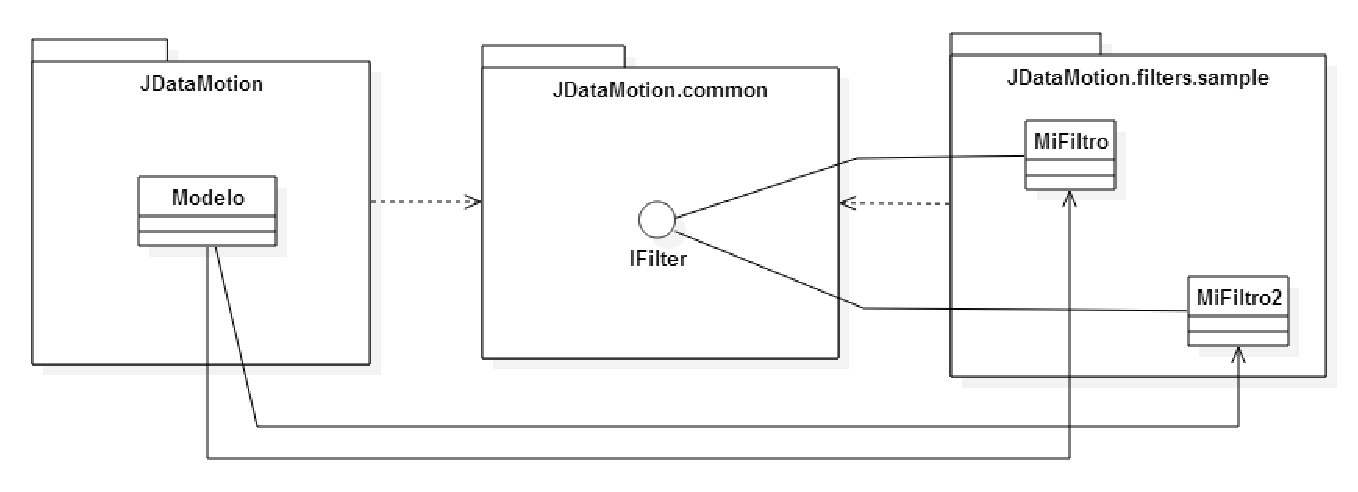
\includegraphics[width=\textwidth,height=\textheight,keepaspectratio]{figuras/disenhoGlobal}
\caption{Deseño global dos 3 módulos que se incluirán dentro do proxecto}
\label{disenhoGlobal}
\end{figure}

A continuación abordaremos o deseño de cada un dos tres módulos implicados neste proxecto.

\section{Deseño de JDataMotion}

Os datos son o punto de partida de todas as funcionalidades deste proxecto. Todo xira arredor do arquivo con información que o usuario importa tras abrir por primeira vez o JDataMotion. O dato debe ser almacenado de xeito adecuado, e accedido só a través dos métodos e clases necesarios, para manter o fluxo de información controlado. A clase que captará, almacenará e distribuirá os datos de cara ás demais clases da aplicación recibirá o nome de Modelo, posto que realmente alberga o modelo da aplicación.

JDataMotion vai ser un programa moi dependente da súa interface de usuario. Os diagramas de dispersión non poden ser visualizados a través dunha simple terminal, e o constante fluxo de datos entre o usuario e o sistema non se pode activar a través dun menú de opcións en termos de usabilidade. Si traballamos co JDataMotion a través dunha interface gráfica multifío como as que Java permite deseñar, a aplicación pode procesar a información ao mesmo tempo que o usuario realiza outras interaccións (ver o modelo, configurar un filtro ou mesmo cancelar a visualización dinámica). Por isto, a clase Vista será un dos artefactos que máis tempo adicaremos a implementar. Vista conterá os ``widgets'' da libraría Swing necesarios para presentar a información ao usuario, e recibir del as novas ordes. Será unha clase complexa e de bastante peso que delegará certas funcións en clases internas ou asociadas.

Só falta unha clase que reciba da Vista as funcionalidades activadas polo usuario e cree un comando que se encargue de realizar o traballo. Esta clase deberá non só disparar o comando, se non que tamén terá que xestionalo, e reaccionar dun xeito específico en caso de que o comando chegue a unha situación de erro. A maioría de comandos influirá directa ou indirectamente sobre o Modelo. A esta clase chamarémoslle Controlador porque a súa responsabilidade será esencialmente esa, a de recibir eventos da Vista e xestionar comandos que actúen de cara ao Modelo. Deste xeito a Vista utilizará a API do Controlador, e quedará exenta de responsabilidade no caso de que se detecten fallas no Modelo.

Acabamos de definir dun xeito explícito cal é o patrón de deseño sobre o que vai xirar toda esta fase do proxecto: o Modelo-Vista-Controlador (MVC). Os patróns de deseño son solucións prácticas a problemas de deseño comúns. En concreto, o Modelo-Vista-Controlador divide o sistema en tres compoñentes coas responsabilidades definidas que xa comentamos anteriormente. A mellor forma de expoñer a aplicación exacta do patrón MVC no noso proxecto é o diagrama da figura \ref{MVC}.

\begin{figure}
\centering
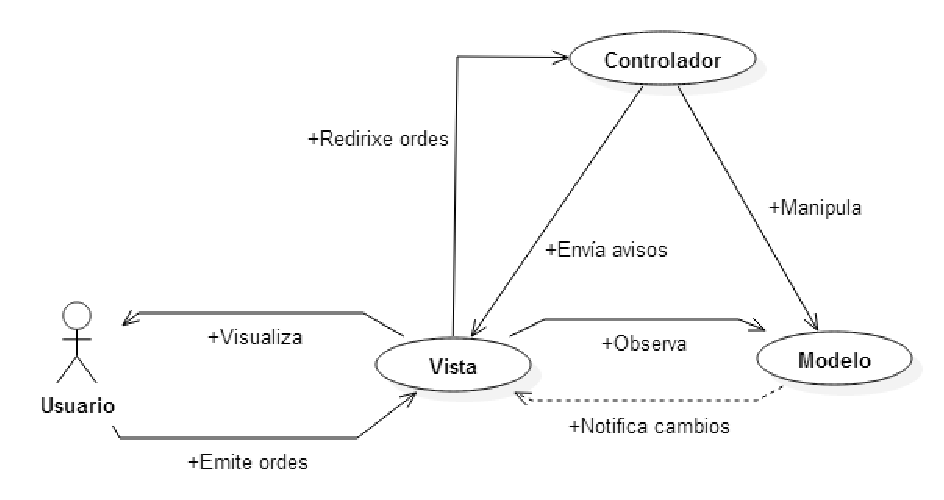
\includegraphics[width=\textwidth,height=\textheight,keepaspectratio]{figuras/MVC}
\caption{Modelo-Vista-Controlador para JDataMotion}
\label{MVC}
\end{figure}

As relacións marcadas cunha liña sólida son asociacións directas (unha clase que actúa de xeito explícito sobre os atributos ou métodos doutra), mentres que a relación marcada cunha liña descontinua representa unha relación indirecta (por exemplo, unha clase que resulta afectada pola actividade doutra). As relacións entre compoñentes detallaranse a continuación.

\begin{itemize}
\item O usuario emite ordes en forma de eventos cara a Vista ao interactuar cos seus botóns e menús.
\item A Vista identifica os eventos que recibe e redirixe cara o Controlador a orde asociada ao evento en cuestión.
\item O Controlador envía un aviso directo á Vista en caso de que a orde que recibe dela levase ao sistema a un estado de erro.
\item O Controlador manipula o Modelo segundo o contido da orde que recibe.
\item O Modelo actúa como entidade observada de cara á Vista. A Vista ten acceso ao Modelo para actualizar a súa aparencia.
\item Do mesmo xeito, que o Modelo sexa observado pola Vista implica que os cambios no modelo serán notificados á Vista, para que esta se actualice no momento do cambio.
\end{itemize} 

Imos documentar máis en profundidade a relación entre a Vista e o Modelo. Comentábamos que a Vista accede ao Modelo para actualizarse cando o desexe, pero ademais o Modelo, cando cambia, notifica á Vista o suceso deste cambio. Temos entón que a Vista actúa como entidade ``observadora'' dun Modelo que é a entidade ``observada''. En esencia, estamos definindo o patrón de deseño Observer.

O patrón de deseño Observer é a mellor resposta que podemos atopar a nivel de deseño para solucionar o problema de manter actualizados ao mesmo nivel o Modelo e a Vista. Se non botásemos man desta solución, teríamos dúas alternativas:

\begin{itemize}
\item Refrescar a vista cada certo intervalo tempo, o cal é ineficiente e seguiría permitindo a posibilidade de que se dese unha incoherencia Vista-Modelo entre refrescos.
\item Permitir ao Modelo que acceda directamente á Vista para invocar un método de actualización, é dicir, asociar directamente a Vista ao Modelo. Isto atenta contra a natureza do Modelo-Vista-Controlador, xa que o Modelo ten que almacenar a información do sistema e abstraerse por completo da Vista ou do módulo que se encargue de representar os seus contidos. Témonos que manter na premisa de que a Vista pode observar ao Modelo e acceder a el para ler datos, pero o Modelo non debe ser consciente da existencia de ningunha Vista.
\end{itemize} 

O patrón Observer pódese aplicar de forma moi sinxela ao noso proxecto. Basta con facer que a Vista implemente a interface \textit{Observer}, de xeito que a obrigue a implementar un método de actualización chamado \textit{update()}, que se disparará cando un obxecto observado cambie o seu estado. Por outra parte, o Modelo só necesita estender a clase \textit{Observable} para ser susceptible de ser observado por un \textit{Observer}. Ao estender esta clase, a Vista xa pode chamar ao método \textit{addObserver(Observer o)} do Modelo, pasándose a ela mesma como parámetro para así incluírse como observadora e ser notificada dos seus cambios.

A asociación dos patróns Modelo-Vista-Controlador e Observer baixo esta forma é bastante común. O libro Pattern-Oriented Software Architecture \cite{pattern-oriented-software-architecture} fai unha boa exposición do que acabamos de mencionar, e aporta o diagrama da figura \ref{MVC-observer} para sintetizar ambos patróns.

\begin{figure}
\centering
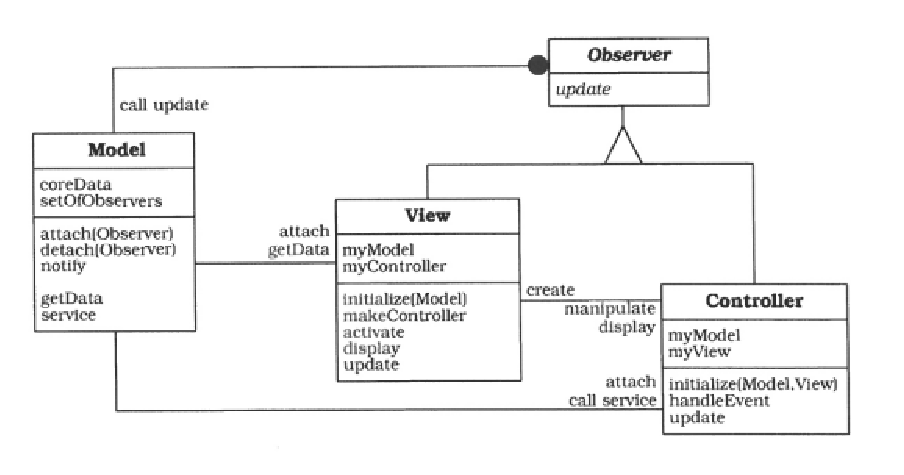
\includegraphics[width=\textwidth,height=\textheight,keepaspectratio]{figuras/MVC-observer}
\caption{Modelo-Vista-Controlador con Observer}
\label{MVC-observer}
\end{figure}

Probablemente a diferencia máis destacable que podemos atopar entre este diagrama e o diagrama que correspondería coa nosa aplicación sería que no noso caso só a Vista implementará a interface \textit{Observer}. O Controlador no noso proxecto non actuará de observador, pois non ten que recibir notificacións ante os cambios do Modelo, xa que de feito el é o responsable directo de todos eses cambios, e non necesita ser notificado de cambios do modelo que non provocase el.

Acabamos de expoñer as 3 clases principais do proxecto e as súas interrelacións, pero debemos ter en conta que cada unha desas clases necesita a axuda doutras que colaboren con ela no obxectivo de cumprir coas súas responsabilidades. O que faremos a continuación será ampliar as 3 entidades básicas do MVC aplicadas ao noso proxecto.

\subsection{Modelo}

O Modelo, como comentábamos, é o responsable de captar e almacenar a información coa que traballamos. A información almacenada clasifícase en 3 conxuntos:

\begin{description}

\item[Instancias:]

Son as tuplas de información coas que se traballa. A estrutura para almacenalas e xestionalas foi reutilizada a partir da API de programación de Weka: a clase Instances. Esta estrutura almacena tanto as propias instancias ou tuplas de información, coma os atributos que levan asociadas. Ademais, contempla toda a información relacionada co atributo: nome, tipo, rango, etc. Esta clase tamén nos facilitará todos os métodos que necesitamos para acceder ou modificar instancias ou atributos. Ademais, a clase Instances de Weka tamén almacena un nome para a relación.

Como veremos, non empregaremos a clase Instances directamente, se non que a estenderemos a través dunha clase á que chamaremos ComparableInstances. A única diferencia entre ambas é que ComparableInstances sobreescribe o método equals(Object o), para determinar que dúas instancias sexan iguais en canto a nome da relación, atributos e tuplas. Isto resultará clave á hora de realizar as probas da aplicación, xa que permitirá verificar que un experimento acada un estado esperado ao aplicarlle unha acción, demostrando a efectividade da mesma.

\item[Filtros:]

O Modelo tamén albergará a secuencia de filtros que utilicemos no noso experimento. Utilizará para isto unha estrutura de tipo lista na que cada novo filtro se engada ao final (se ben é posible cambiar a posición dos filtros e polo tanto a orde da súa aplicación).

Para seren útiles de cara ao Modelo, os filtros deben de conter unha pequena porción de lóxica que a interface IFilter non pode incorporar. Por isto, o Modelo tratará de encapsular cada IFilter co que traballe dentro dun FilterHandler. O FilterHandler só é un manexador da interface que contén, pero con outros campos necesarios como o índice do atributo sobre o que opera o filtro, ou un parámetro de bandeira que indica si o filtro está seleccionado. En canto a métodos, o FilterHandler tamén ofrece ao Modelo un conxunto de procedementos prácticos para traballar co filtro en cuestión.

\item[Outros elementos:]

O Modelo tamén almacena outros datos máis discretos acerca do experimento, como son os índices de atributo temporal e nominal que se empregarán na visualización, a dirección ao ficheiro de orixe e o resumo SHA1 do mesmo (para posibilitar a creación e restauración de sesións).

\end{description}

\begin{figure}
\centering
\centerline{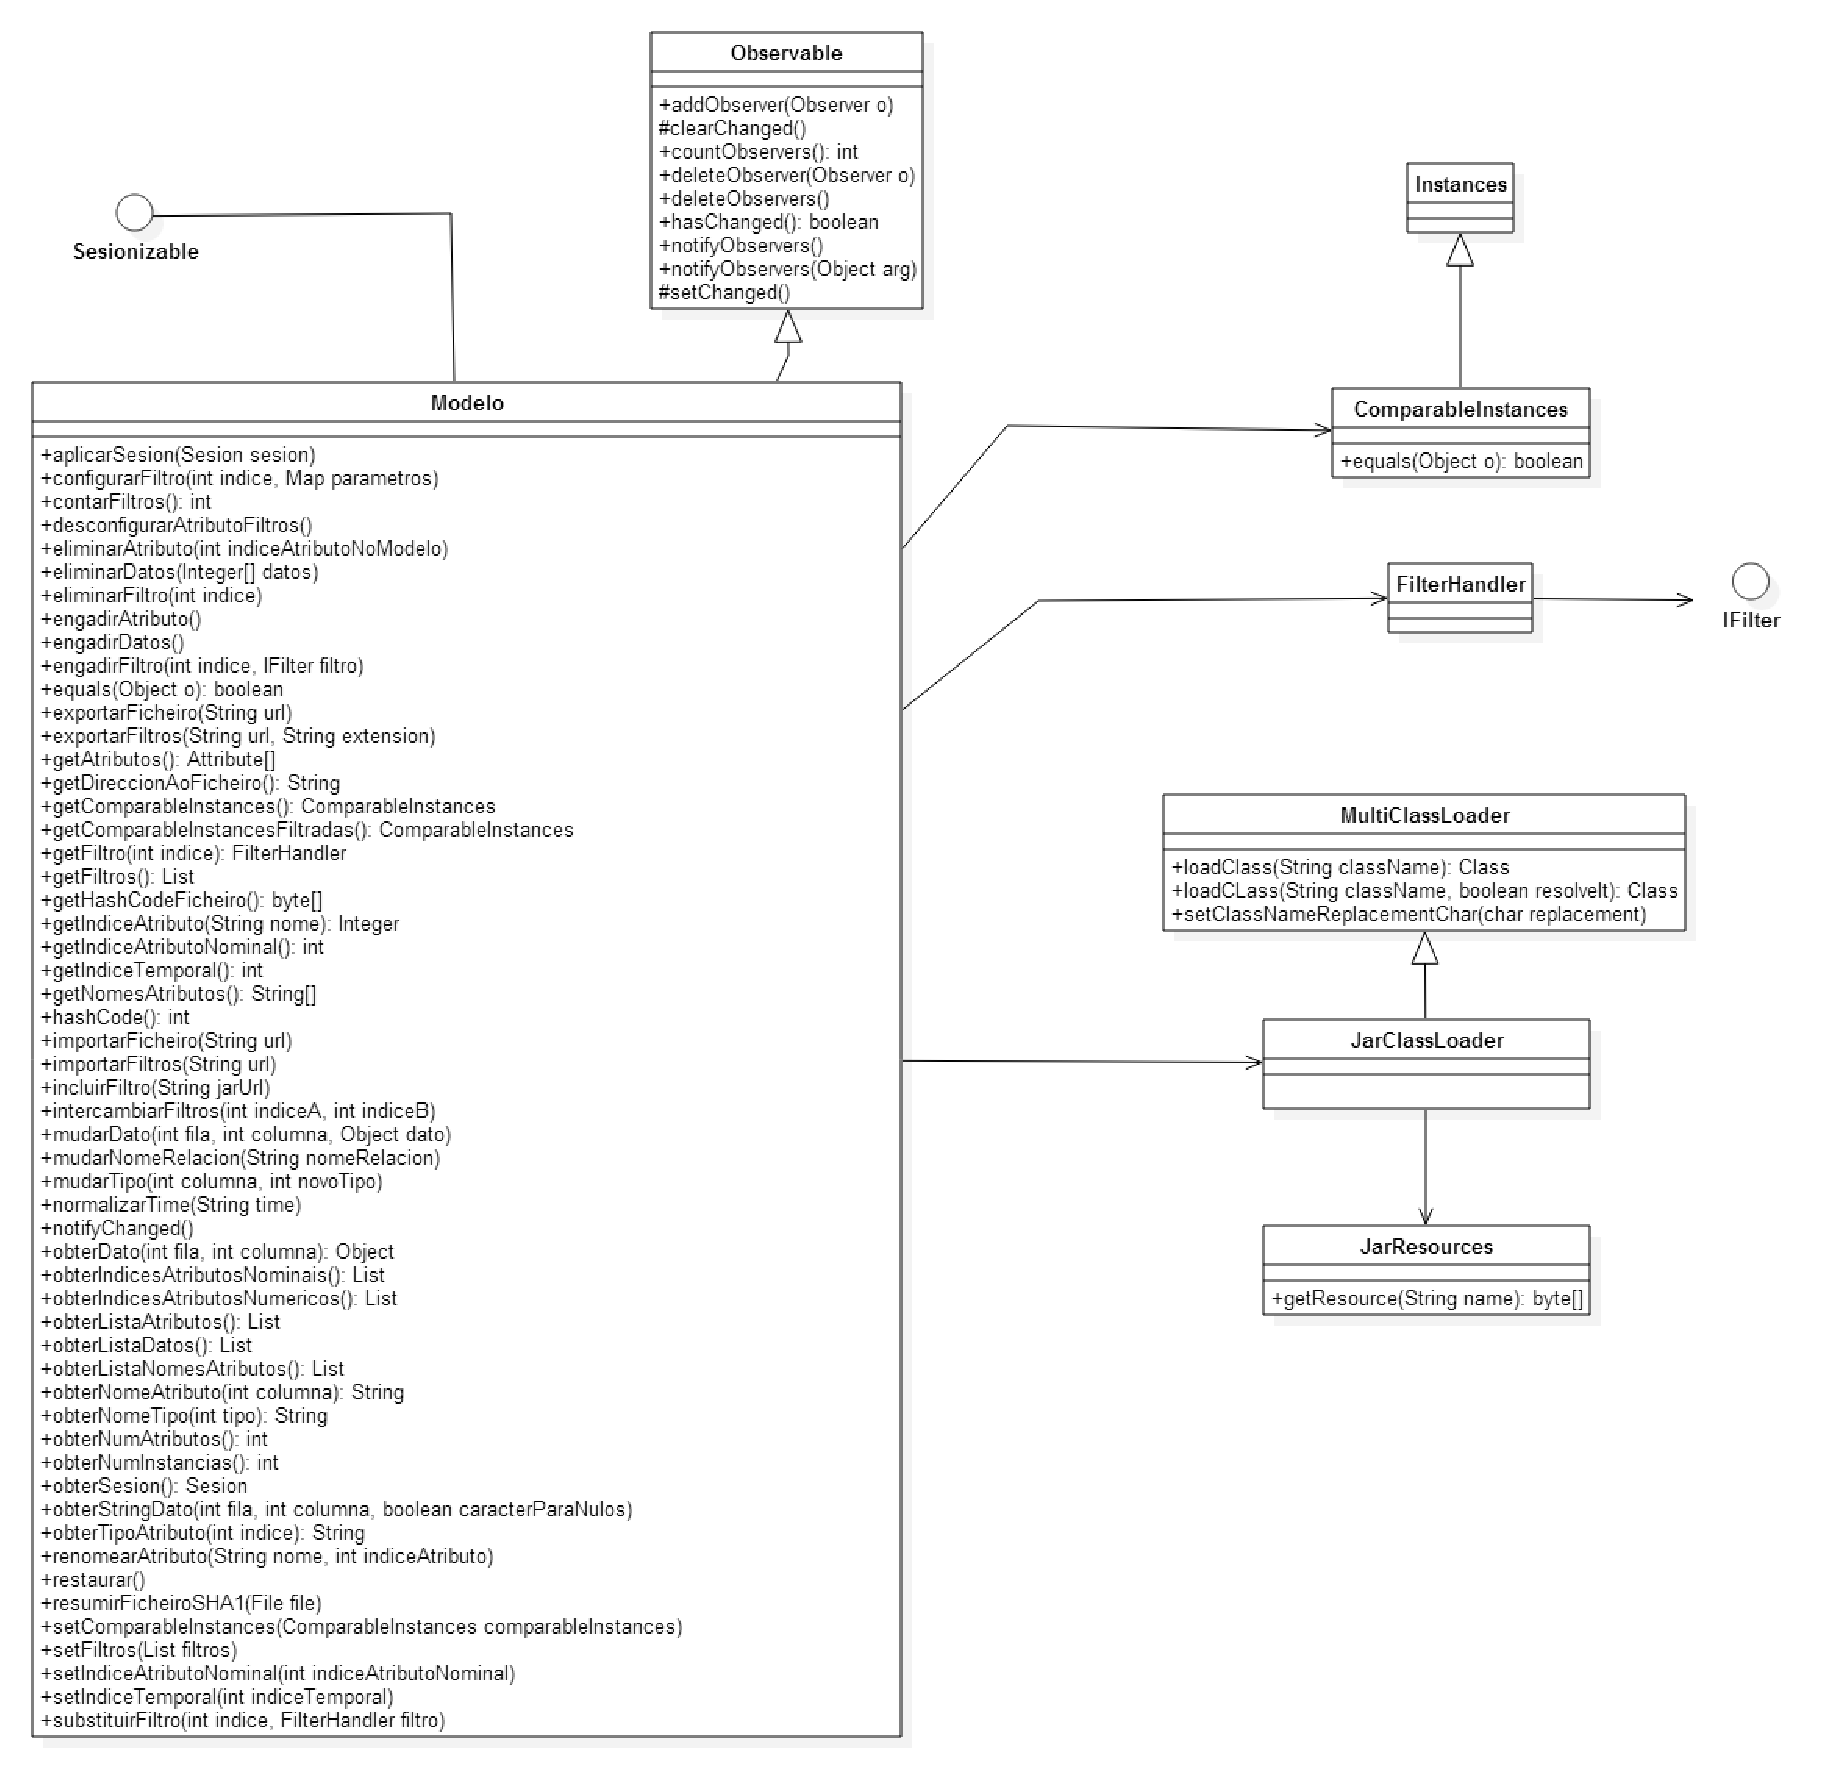
\includegraphics[width=1.4\textwidth,height=1.4\textheight,keepaspectratio]{figuras/UMLmodelo}}
\caption{Diagrama de clases do modelo}
\label{UMLmodelo}
\end{figure}

A continuación expoñeremos e comentaremos o deseño da sección Modelo. O diagrama de clases preséntase na figura \ref{UMLmodelo}. O Modelo debe contar cunha gran batería de métodos útiles para o Controlador. Isto significa que se debe crear un número suficiente de métodos concretos para as necesidades de almacenamento de datos que vaia ter o proxecto, pois as responsabilidades do Controlador non contemplan o traballo directo con unidades de información pesadas como son as ComparableInstances. Isto é, polo xeral será preferible esixirlle ao Modelo unha tupla de información determinada, ca pedirlle todas as ComparableInstances e mesturar dentro do Controlador a xestión de eventos coa procura dunha tupla dentro das instancias totais. En definitiva, en certa medida o Modelo debe ofrecer ao Controlador unha API de programación que atenda ás súas necesidades individuais.

O Modelo, como xa comentáramos anteriormente, estendía a clase Observable (neste caso escolleremos a do paquete java.util). Ademais implementará a interface Sesionizable, que permitirá que os seus campos sexan almacenados nunha sesión para ser recuperados posteriormente. Os dous métodos que deberá implementar serán obterSesion(), que obligará ao Modelo a devolver unha SesionModelo cos datos que desexa salvar, e aplicarSesion(Sesion sesion), que tratará de recuperar a sesión a partir da SesionModelo previamente obtida.

Os datos do Modelo que desexaremos salvar son:

\begin{itemize}
\item A dirección ao ficheiro de orixe do experimento
\item As cabeceiras do experimento (o conxunto dos atributos que manexa).
\item O índice do atributo que representa a temporalidade.
\item O resumo ou hash do ficheiro de orixe, para protexer a integridade.
\item O nome da relación coa que se está a traballar.
\item O índice do atributo nominal (atributo de clase) que se está a empregar.
\end{itemize}

Un dos métodos máis destacables do Modelo é notifyChanged(). Este método comproba que o obxecto en cuestión cambiou o seu estado, e en caso afirmativo invoca ao método update(Observable o, Object arg) de todos cantos obxectos estean observando ao Modelo. A comprobación de que o Modelo cambiou realízase cos métodos setChanged() e clearChanged() herdados da clase Observable, que activan ou desactivan unha variable de bandeira. O método setChanged() será chamado polo Modelo cada vez que este acade un novo estado que deba ser notificado (por exemplo, que se engadise unha nova instancia). A continuación, cando o Controlador invoque o notifyChanged() do Modelo comprobarase a bandeira, si esta está activada invocarase ao update(Observable o, Object arg) dos observadores, e a continuación con clearChanged() volverase a desactivar, indicando que non houbo cambios dende a última actualización. O Modelo tamén contén un método reset() que reinicia a súa actividade previa cada vez que comeza un novo experimento.

Outras das clases das que se valerá o Modelo para realizar a súa labor é JarClassLoader. Esta clase estende a MultiClassLoader e utiliza a JarResources para permitir cargar en tempo de execución proxectos .jar xa compilados, posibilitando a importación dinámica de filtros. A clase JarClassLoader será estática e con visibilidade suficiente para permitir que a Vista a use, xa que a vai necesitar para ler directamente dende o directorio onde o Modelo almacena os filtros en .jar que importa.

\subsection{Controlador}

A continuación expoñeremos e comentaremos o deseño da sección Controlador. O diagrama de clases preséntase na figura \ref{UMLcontrolador}. O Controlador é o motor da aplicación, a clase involucrada na maioría das transaccións que afectan ao experimento. A súa tarefa principal é recibir o fluxo de eventos que a Vista notifica, e realizar a operación axeitada en consecuencia. Si a operación require dun procesamento complexo dos datos, o Controlador delegará na lóxica do Modelo para obter o resultado que desexa.

\begin{figure}
\centering
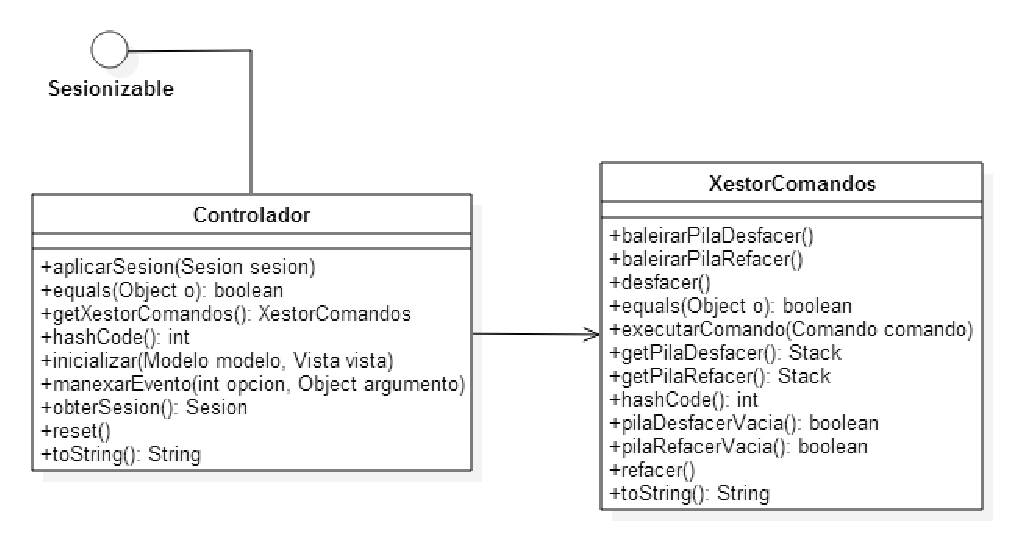
\includegraphics[width=\textwidth,height=\textheight,keepaspectratio]{figuras/UMLcontrolador}
\caption{Diagrama de clases do controlador}
\label{UMLcontrolador}
\end{figure}

O Controlador, como motor da aplicación, contén o método inicializar, que recibe unha Vista e un Modelo para comezar a desempeñar as súas funcións. Tamén contén un método reset() que reinicia a súa actividade previa cada vez que comeza un novo experimento.

A pesar de que o Controlador recibe os eventos a través do seu método máis importante: manexarEvento(int opcion, Object argumento). Para procesalos, botará man dunha clase auxiliar chamada XestorComandos, que expoñeremos a continuación. A especificación de que eventos e argumentos pode recibir este método amósase na figura \ref{manexarEvento}. Esta especificación xa figura no código fonte como o JavaDoc do método, de forma que durante a implementación teñamos acceso áxil á especificación deste método, cando estemos configurando dende a Vista as chamadas a este método do Controlador.

\begin{figure}
\centering
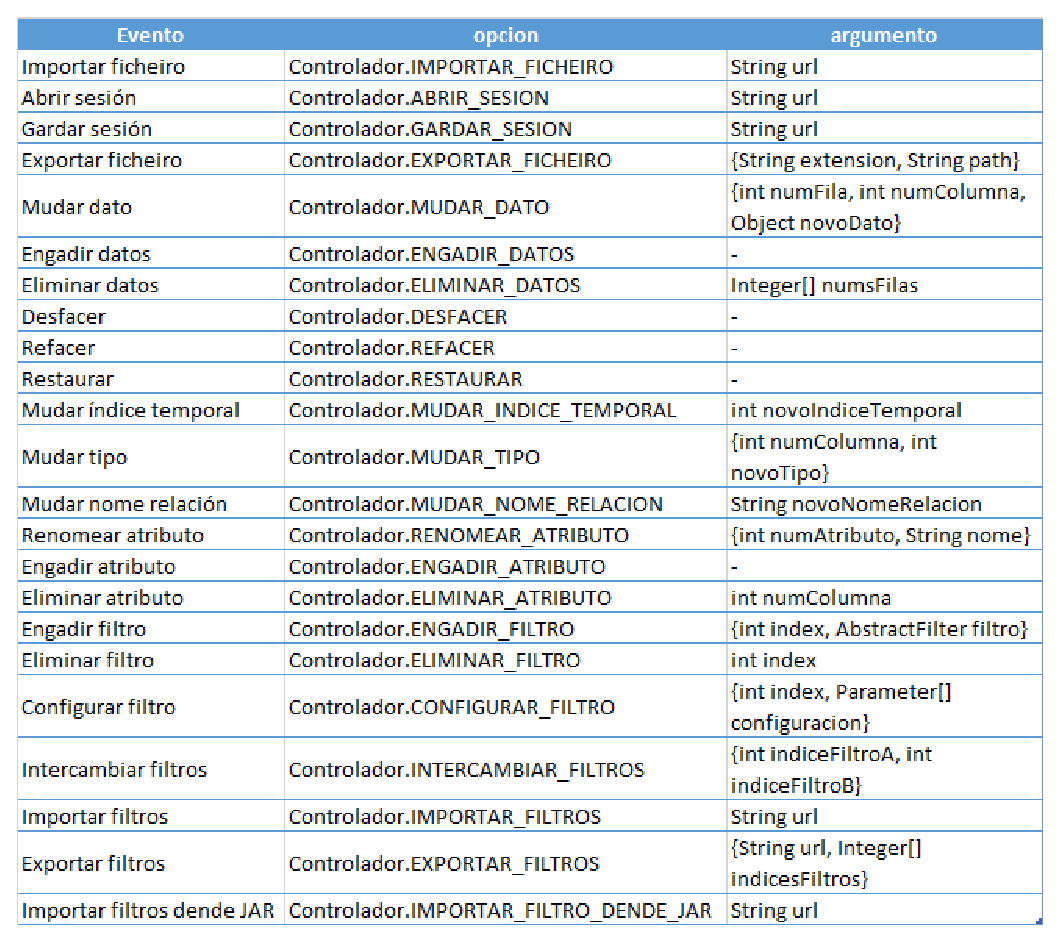
\includegraphics[width=\textwidth,height=\textheight,keepaspectratio]{figuras/manexarEvento}
\caption{Inputs do método manexarEvento}
\label{manexarEvento}
\end{figure}

O parámetro opción é un enteiro que representa ao evento, e todos os valores que pode tomar son constantes declaradas estaticamente na propia clase Controlador. O parámetro argumento debe ser de un tipo ou outro en función da opción escollida. Nos casos nos que na especificación figure unha lista de tipos entre corchetes ({String a, Integer b}), referirase a un array de obxectos ou Object[] (primeiro elemento de tipo String, segundo elemento de tipo Integer).

A clase Controlador recibe eventos a través de manexarEvento, e invoca a un método do XestorComandos para procesalo. Este método non será outro que executarComando(Comando comando). A este método o Controlador debe pasarlle unha instancia do comando que queira procesar, de xeito que a clase Controlador está traducindo eventos que recibe da Vista en comandos que envía ao XestorComandos. Entre as responsabilidades do Controlador tamén está a de recoller as excepcións que poda devolver o XestorComandos, e procesalas adecuadamente (por exemplo ordenándolle á Vista que informe do erro).

Ás veces os eventos non se traducen a comandos, se non que se procesan directamente polo controlador, por exemplo no caso de que o evento desencadee a necesidade de acceder ao Modelo e máis á Vista para aplicar sesións neles. O proceso de tradución de cada evento explícase a continuación:

\begin{description}
\item[IMPORTAR\_FICHEIRO:] Envía ao XestorComandos unha instancia de ComandoImportarFicheiro
\item[ABRIR\_SESION:] Carga os filtros personalizados da carpeta filters no ClassLoader (por si a nova sesión botase man deles) e acto seguido aplica na Vista, no Modelo e no propio Controlador cadansúa sesión contida no ficheiro.
\item[GARDAR\_SESION:] Solicita as sesións (co método obterSesion(), da interface Serializable) de Modelo, Vista e a do propio Controlador para almacenalas nun ficheiro.
\item[EXPORTAR\_FICHEIRO:] Envía ao XestorComandos unha instancia de ComandoExportarFicheiro.
\item[MUDAR\_DATO:] Envía ao XestorComandos unha instancia de ComandoMudarDato.
\item[ENGADIR\_DATOS:] Envía ao XestorComandos unha instancia de ComandoEngadirDatos.
\item[ELIMINAR\_DATOS:] Envía ao XestorComandos unha instancia de ComandoEliminarDatos.
\item[DESFACER:] Invoca ao método desfacer() de ManexadorEventos.
\item[REFACER:] Invoca ao método refacer() de ManexadorEventos.
\item[RESTAURAR:] Envía ao XestorComandos unha instancia de ComandoRestaurar.
\item[MUDAR\_INDICE\_TEMPORAL:] Envía ao XestorComandos unha instancia de ComandoMudarIndiceTemporal.
\item[MUDAR\_TIPO:] Envía ao XestorComandos unha instancia de ComandoMudarTipo.
\item[MUDAR\_NOME\_RELACION:] Envía ao XestorComandos unha instancia de ComandoMudarNomeRelacion.
\item[RENOMEAR\_ATRIBUTO:] Envía ao XestorComandos unha instancia de ComandoRenomearAtributo.
\item[ENGADIR\_ATRIBUTO:] Envía ao XestorComandos unha instancia de ComandoEngadirAtributo.
\item[ELIMINAR\_ATRIBUTO:] Envía ao XestorComandos unha instancia de ComandoEliminarAtributo.
\item[ENGADIR\_FILTRO:] Envía ao XestorComandos unha instancia de ComandoEngadirFiltro.
\item[ELIMINAR\_FILTRO:] Envía ao XestorComandos unha instancia de ComandoEliminarFiltro.
\item[CONFIGURAR\_FILTRO:] Envía ao XestorComandos unha instancia de ComandoConfigurarFiltro.
\item[INTERCAMBIAR\_FILTROS:] Envía ao XestorComandos unha instancia de ComandoIntercambiarFiltros.
\item[IMPORTAR\_FILTROS:] Envía ao XestorComandos unha instancia de ComandoImportarFiltros.
\item[EXPORTAR\_FILTROS:] Envía ao XestorComandos unha instancia de ComandoExportarFiltros.
\item[IMPORTAR\_FILTROS\_DENDE\_JAR:] Envía ao XestorComandos unha instancia de ComandoImportarFiltrosDendeJAR.
\end{description}

Cada vez que se termina de executar un comando, o Controlador solicita ao Modelo a execución de notifyChanged, para que en caso de que este último sufrise modificacións con motivo da execución do comando, a Vista sexa capaz de plasmar a nova información. Xuntando a relación evento-comando coa aplicación do patrón Observer conseguimos que o noso sistema se manteña sempre actualizado ante calquera cambio no Modelo, xa que a causa dos cambios debe pasar polo método manexarEvento do Controlador, e este método sempre remata chamando a notifyChanged. Ambas entidades manteranse sincronizadas sen recorrer a esperas activas ou refrescos innecesarios. Para apreciar mellor as interaccións durante todo este proceso, a figura \ref{DScomandos} contén un diagrama de secuencia que o ilustra.

\begin{figure}
\centering
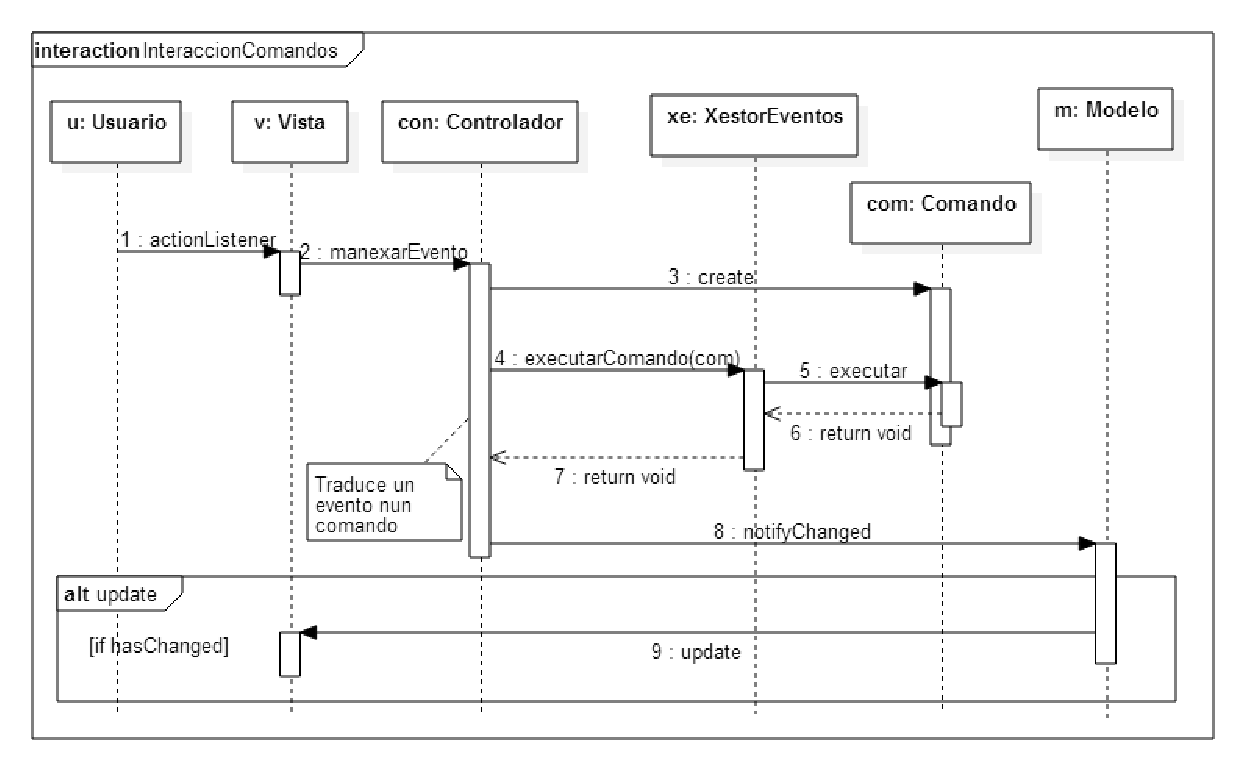
\includegraphics[width=\textwidth,height=\textheight,keepaspectratio]{figuras/DScomandos}
\caption{Diagrama de secuencia evento-notificación}
\label{DScomandos}
\end{figure}

Os comandos que o Controlador emite ao XestorComandos son a forma de manter controladas as transaccións que alteran ao Modelo. Os comandos seguen unha xerarquía que se expón na figura \ref{xerarquiaComandos}.

\begin{figure}
\centering
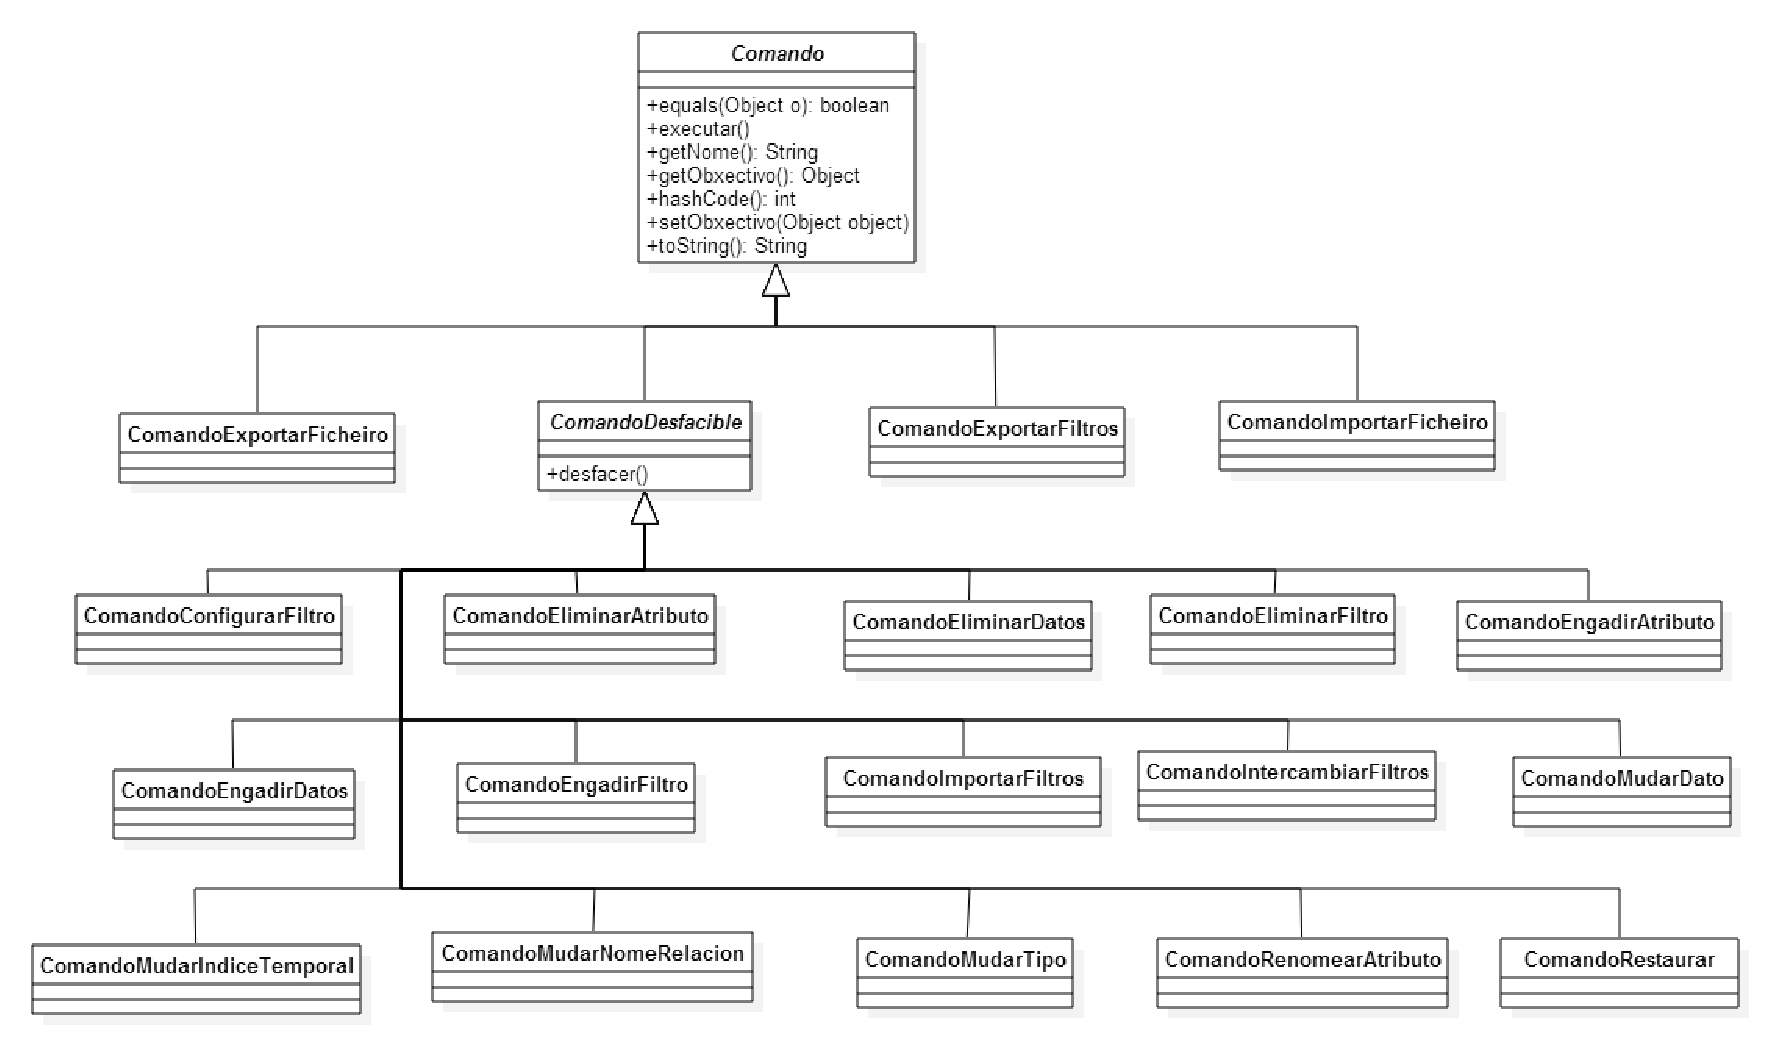
\includegraphics[width=\textwidth,height=\textheight,keepaspectratio]{figuras/xerarquiaComandos}
\caption{Xerarquía de comandos}
\label{xerarquiaComandos}
\end{figure}

Todos os comandos realizan a súa función no método executar(). O construtor da superclase Comando sempre debe recibir un Modelo (ao que tratará co nome de obxectivo). Este obxectivo, que poderemos recuperar por medio de getObxectivo(), é o que se terá que modificar no método executar(). O outro parámetro que debe recibir o construtor de Comando é o nome do comando en cuestión, que poderemos recuperar por medio de getNome().

A maioría de Comandos que o Controlador pode elixir para pasarlle ao XestorComandos son clases que estenderán a superclase ComandoDesfacible. Cando un XestorComandos recibe un Comando que deriva de ComandoDesfacible, almacenarao na pila de desfacer tras a súa correcta execución. Deste xeito, si o Controlador recibe un evento solicitando desfacer o último comando, executará o método desfacer() do XestorComandos directamente. Análogamente poderanse refacer comandos desfeitos. Cabe destacar que os eventos Desfacer e Refacer non xeran comando algún, se non que se tratan chamando ao método desfacer() ou refacer() directamente. O diagrama de secuencia destes dous eventos podémolo observar na figura \ref{xerarquiaComandos}.

\begin{figure}
\centering
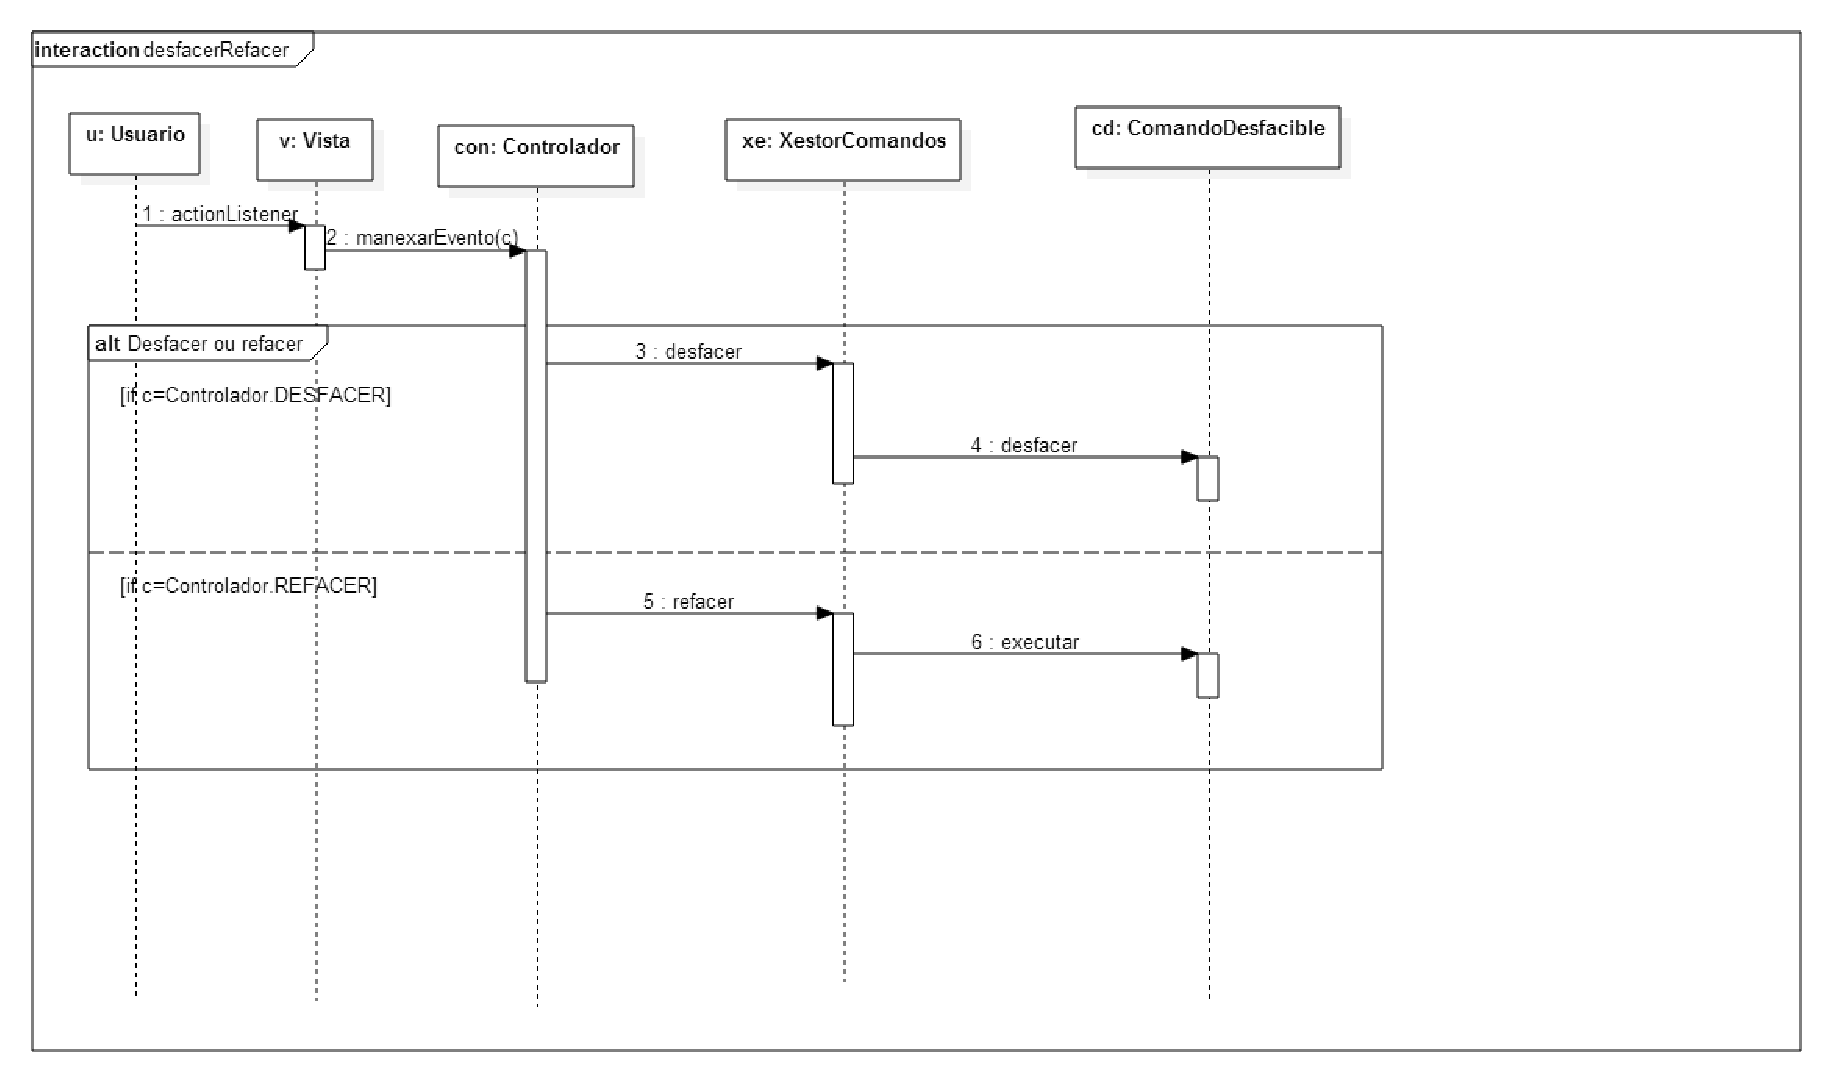
\includegraphics[width=\textwidth,height=\textheight,keepaspectratio]{figuras/desfacerRefacer}
\caption{Diagrama de secuencia dos eventos desfacer e refacer}
\label{desfacerRefacer}
\end{figure}

Do mesmo xeito que se debe implementar o método executar() para todos os comandos atendendo ao seu propósito, no caso dos ComandosDesfacibles tamén debemos implementar o método desfacer(), otorgándolle a este un comportamento que permita inverter os efectos do método executar(). A coherencia entre os procedementos executar() e desfacer() é unha responsabilidade á hora de programar comandos útiles para JDataMotion.

Existe un último grupo de comandos que comentar, e é aquel composto por comandos que aínda que estenden a clase Comando, non estenden a clase ComandoDesfacible. Estes comandos son executados sen posibilidade de entrar ou saír das pilas pilaDesfacer ou pilaRefacer que contén o XestorComandos. Trátase dos seguintes comandos:

\begin{description}

\item[ComandoExportarFicheiro:]

A exportación dun experimento supón a creación dun novo ficheiro no sistema. Esta acción non debe poder desfacerse, xa que atentaría contra a propia finalidade do comando, que é a de salvar permanentemente os datos do experimento no disco duro.

\item[ComandoExportarFiltros:]

Baixo a mesma filosofía anterior, os accesos a disco carecen da necesidade de ser reversibles.

\item[ComandoImportarFicheiro:]

O inicio dun novo experimento reinicia por completo os datos do sistema. Non se deben manter as pilas do XestorComandos dun experimento a outro.

\item[ComandoImportarFiltrosDendeJAR:]

Este comando realiza unha copia do ficheiro JAR nos directorios da aplicación e carga as súas clases no ClassPath de Java. Mentres o JDataMotion se execute, este ficheiro estará en uso e non se poderá eliminar.

\end{description}

O Controlador, do mesmo xeito ca o Modelo, implementa a interface Sesionizable, que permitirá que os seus campos sexan almacenados nunha sesión para ser recuperados posteriormente. Os dous métodos que deberá implementar serán obterSesion(), que obligará ao Controlador a devolver unha SesionControlador cos datos que desexa salvar, e aplicarSesion(Sesion sesion), que tratará de recuperar a sesión a partir da SesionControlador previamente obtida.

Os datos do Controlador que desexaremos salvar son:

\begin{itemize}
\item O xestor de comandos, con todos os comandos das pilas desfacer e refacer. Cos da primeira poderemos restaurar o modelo de datos a partir das instancias iniciais do experimento.
\end{itemize}

\subsection{Vista}

A continuación expoñeremos e comentaremos o deseño da sección Vista. O diagrama de clases preséntase na figura \ref{UMLvista}, e contén un conxunto de clases (algunhas privadas e internas á clase Vista) que participan e comparten certas responsabilidades con ela. A sección Vista ten varios cometidos nesta aplicación:

\begin{itemize}
\item Implementar a interface gráfica da aplicación, as súas ventás e todos os widgets necesarios para permitir a interacción co usuario.
\item Inicializar, configurar e xestionar o conxunto de diagramas de dispersión da aplicación. 
\item Implementar métodos de reprodución sobre o conxunto de diagramas de dispersión.
\end{itemize}

Imos comentar as clases do diagrama anteriormente mencionado, así como as súas relacións e métodos.

\begin{description}

\item[Vista:] \hfill
É a clase de partida da sección, a primeira en ser instanciada. Estende á clase JFrame, que é o widget da librería Swing empregado para representar as ventás, pois a clase Vista é efectivamente unha ventá sobre a que se colocan outros widgets. Implementará 3 interfaces que a obrigarán a darlle corpo a unha serie de métodos:
\begin{description}
\item[Observer:] \hfill
De acordo co patrón Observer, a clase Vista vai ser a clase observadora, neste caso da clase observable Modelo. Isto significa que cando o Modelo cambie algún aspecto do seu contido e chame ao método de actualización, a clase Vista executará o método update(Observable o, Object arg), sendo neste caso os argumentos da función de pouca utilidade, xa que o obxecto observado será sempre o Modelo, e non se necesitarán argumentos. O corpo deste método tratará de refrescar toda a interface gráfica, pintando outra vez os contedores dos 3 menús: Modelo, Filtros e Visualización.
Refrescar o menú Modelo e Filtros non será normalmente un proceso custoso, pero co terceiro, no caso de que a matriz de diagramas de dispersión que se quere visualizar teña uns 1000 diagramas ou máis, a latencia comezará a facerse notable. Intentaremos combater esta problemática alixeirando o proceso na medida do posible, e a partir de aí comezaremos a traballar en termos de usabilidade para facer o proceso menos pesado de cara ao usuario.
Algunhas medidas para isto comentaranse a continuación, pero a primeira delas que adoptamos consistirá en bloquear o refresco deste menú ata que se cambie á lapela de Visualización, permitindo varias edicións nos menús Modelo e Filtros que eviten a latencia de refresco deste último menú.
\item[Sesionizable:] \hfill
Analogamente ás clases Modelo e Controlador, a clase Vista tamén pode gardar o seu contido (e o das clases que dependan dela) dentro dunha sesión. A interface Sesionizable permitirá que os seus campos sexan almacenados nunha sesión para ser recuperados posteriormente. Os dous métodos que deberá implementar serán obterSesion(), que obligará á Vista a devolver unha SesionVista cos datos que desexa salvar, e aplicarSesion(Sesion sesion), que tratará de recuperar a sesión a partir da SesionVista previamente obtida.

Os datos da Vista que desexaremos salvar, e que ampliaremos a continuación, son os seguintes:

\begin{itemize}
\item O conxunto de diagramas de dispersión que foron marcados para visualizar.
\item A orde de visualización seleccionada para a reprodución dos datos.
\item A lonxitude da estela.
\item A cor da estela.
\item O paso en milisegundos utilizado na reprodución.
\item A fórmula da distancia configurada
\end{itemize}

\item[PropertyChangeListener:] \hfill
Esta interface permite que a Vista reaccione ante o cambio dalgunha propiedade noutra instancia, en concreto utilizaremos esta capacidade para ``escoitar'' os cambios no ManexadorScatterPlots da propiedade ``estadoReprodutor''. Deste xeito, a barra cos botóns de reprodución implementados na Vista poderá manterase actualizada ante calquera cambio no reprodutor. Esta sincronización producirase no corpo do método propertyChange(PropertyChangeEvent evt).
\end{description}

Outros métodos da Vista, aparte dos asociados ás interfaces, que merece a pena destacar son:

\begin{description}
\item[doEditProperties(Component c):] \hfill
Visualiza dentro do compoñente c (por exemplo a propia Vista) un editor de parámetros para diagramas de dispersión. É dicir, abre un cadro de diálogo onde se poden seleccionar cores de fondo dos diagramas, forma e cores dos puntos, fonte das marcas dos eixos, etc. Toda a información recollida neste diálogo é primeiramente almacenada en ficheiro como configuración de usuario, e a continuación invócase un refresco da configuración gráfica dos diagramas, que accede a ficheiro para utilizar sempre a última configuración gráfica a nivel global.
\item[amosarDialogo(String mensaxe, int tipo):] \hfill
Método invocado polo controlador para visualizar mensaxes de erro que poidan xurdir.
\item[getControlador():] \hfill
Este método é de acceso protected. Só desexamos que se acceda a el para os test de proba para acceder ao controlador (pois o Controlador instánciase na Vista).
\item[getRecursosIdioma():] \hfill
Devolve a instancia de ResourceBundle (unha clase parecida a un HashMap) que permite internacionalizar os textos da aplicación visibles ao usuario. Cada clave introducida nesta estrutura devolve un valor en función do idioma do sistema.
\item[inicializar(Modelo modelo, boolean visualizar):] \hfill
Método que usamos para iniciar a Vista integrándoa co modelo e cun Controlador.
\item[reiniciarAplicacion():] \hfill
Pecha e arranca de novo o JDataMotion. Isto empregarase ao cambiar o idioma ou outros parámetros que precisen dun reinicio.
\item[reset():] \hfill
Reinicia os campos da Vista (por exemplo, ao importar un novo ficheiro ou abrir unha nova sesión).
\item[setScatterPlotsBackground():] \hfill
Este método asigna a cor de fondo do menú de Visualización. Non recibe a cor como parámetro, xa que a lee da configuración de usuario, almacenada no ficheiro de configuración persoal.
\end{description}

\item[GraphicConfigurationManager:] \hfill
É unha clase composta por unha batería de métodos estáticos para ler e escribir parámetros de usuario. Os parámetros de usuario poden ser o idioma, as cores de fondo do menú Visualización, o formato dos puntos dos diagramas, etc. e almacénanse en ficheiro (configuracion.properties). Existe un ficheiro de configuración interno por defecto (default\_config.properties) para todos os parámetros de usuario que aínda non fosen definidos. Os tipos de datos que estes métodos permiten tanto ler coma escribir son:

\begin{itemize}
\item Boolean, representando no ficheiro true coma `y' e false coma `n'
\item Color, representando no ficheiro o seu formato RGB con comas entre cada compoñente.
\item Double, representando no ficheiro o número coma un String.
\item Font, representando no ficheiro o nome da fonte, seguido dun punto e os atributos (PLAIN, ITALIC, BOLD ou BOLD+ITALIC), e seguido dunha coma e o tamaño da fonte.
\item ListColor, representando cada cor co formato dos parámetros Color, e separando cada un deles entre sí por medio de `|'.
\item ListShape, representando cada forma con `regular' no caso dun polígono regular e `star' no caso dunha estrela, seguido dunha coma e o número de vértices da forma, e á súa vez separando cada unha das formas entre sí por medio de `|'.
\end{itemize}

Todas as clases da vista accederán a estes métodos estáticos para obter ou modificar a última configuración gráfica almacenada. Debido a isto, os métodos públicos e privados que almacenen ou lean cada propiedade deberán ter o modificador synchronized para evitar inconsistencias no sistema.

\item[TarefaProgreso:] \hfill
É unha das clases que mellora a experiencia de usuario durante a latencia que implica visualizar certo número de diagramas de dispersión. Esta clase iníciase xunto cun JProgressBar (o widget de Swing para as barras de progreso). Despois, establécese un número de puntos totais ou finais con setEnd(int end) e chámase a acumulate(int cantidade) cada vez que avancemos un número ``cantidade'' de puntos na nosa tarefa. A medida que os puntos aumenten, o método doInBackground() incrementará o valor da barra de progreso, ata chegar ao total estipulado.
Para conseguir este comportamento é vital que TarefaProgreso estenda SwingWorker, xa que se non o Event Dispatch Thread (o fío que se encarga de visualizar e actualizar a interface gráfica) quedaría bloqueado ata que a tarefa rematase (e a barra de progreso pasaría do 0\% ao 100\% directamente). A clase SwingWorker executa o seu método doInBackground() mantendo o EDT activo, así que no seu corpo será onde programemos os incrementos da barra de progreso.

\item[ManexadorScatterPlots:] \hfill
Esta clase supón a mellor aliada que ten a Vista para xestionar os diagramas de dispersión. A Vista instancia un ManexadorScatterplots cada vez que volve a pintar o menú de Visualización, e facilítalle toda a configuración necesaria para que poda realizar o seu traballo. O seu cometido é iniciar os diagramas de dispersión (nun formato matricial), configuralos e almacenalos para que a vista poda solicitalos cando os necesite. Tamén ofrece á Vista unha serie de métodos de reprodución, coordinándose con outras clases para conseguir isto.

A reprodución será un proceso concorrente que non debe bloquear outras funcionalidades. Mentres a visualización se desenvolve, débese poder avanzar cara adiante ou cara atrás cos botóns, cambiar a posición co desprazador ou por suposto pausar a reprodución. Todas estas interaccións van involucrar elementos compartidos coma atributos ou métodos de clases (o instante de tempo no que me atopo, o número de puntos que se visualizaron, etc.), así que para manter a consistencia do sistema será habitual declarar métodos ou bloques de execución coa partícula ``synchronized''.

A continuación describiremos os métodos fundamentais de ManexadorScatterplots:

\begin{description}
\item[addPropertyChangeListener(PropertyChangeListener propertyChangeListener):] \hfill
Engade unha clase que implemente PropertyChangeListener á lista de ``listeners'', para notificarlle calquera cambio nunha propiedade. Neste caso o obxecto que vai estar escoitando vai ser a Vista, e quen a vai avisar de cambios no reprodutor (play, pause) vai ser unha instancia de TarefaPlay, unha clase colaboradora de ManexadorScatterPlots.
\item[aplicarConfiguracionGraficaScatterPlots():] \hfill
Este método aplica en todos os diagramas de dispersión a súa configuración gráfica (cores, fontes de marcas nos eixos, formato dos puntos debuxados, etc.). Non recibe ningún parámetro porque sempre colle a configuración gráfica de usuario almacenada no momento actual, léndoa dende o ficheiro de configuración.
\item[columnaScatterPlotsVacia(int columna):] \hfill
Indica si a columna de índice dado dentro da matriz de diagramas de dispersión está baleira. Isto significaría que non se solicitou a visualización de ningún diagrama que represente o atributo de índice dado no eixo de abscisas.
\item[contarJFramesVisibles():] \hfill
Devolve o número de diagramas de dispersión que foron ampliados nunha ventá (JFrame) aparte.
\item[createPropertiesPopupMenu():] \hfill
Devolve un menú contextual (JPopupMenu) cunha soa opción, ``Propiedades''. Esta opción permite editar a configuración gráfica de usuario. Esta opción está por defecto no menú contextual de todos os diagramas de dispersión, pero a Vista necesitará dispor del para engadirllo tamén ao propio contedor do menú Visualización, aínda que non haxa diagramas nel aínda.
\item[cubrirConScatterPlot(int i, int j, List indicesNumericos, int indiceAtributoNominal):] \hfill
Posiblemente un dos métodos máis importantes desta clase. Primeiro comprobará que na matriz de diagramas de dispersión o elemento (i, j) fose realmente marcado para visualizar. En caso afirmativo, instancia un ScatterPlot e colócao na matriz nesa posición. O parámetro ``indicesNumericos'' úsase para localizar facilmente que atributos son numéricos, e polo tanto susceptibles de ser representados, sen ter que iterar ao longo de todos os atributos.
Este método será invocado na Vista, dentro do método interno que volve a pintar o menú de visualización, para encher os ocos da matriz de diagramas nos casos que sexa necesario. Para aliviar a espera en caso de matrices de diagramas de certo tamaño, este método será invocado dende un fío que non interrompa o resto da execución. Ademais, a medida que se creen, estes iranse visualizando, así que comezaremos a invocar este método pasándolle as posicións da esquina inferior esquerda da matriz, que é a zona que se visualiza primeiro dentro do scroll que ten este menú. Deste xeito, resultará menos tenso esperar a que se encha a barra de progreso si xa podemos ver algúns dos diagramas que escollemos.
\item[filaScatterPlotsVacia(int fila):] \hfill
Indica si a fila de índice dado dentro da matriz de diagramas de dispersión está baleira. Isto significaría que non se solicitou a visualización de ningún diagrama que represente o atributo de índice dado no eixo de ordenadas.
\item[freeze():] \hfill
Conxela a reprodución. O estado conxelado implica que a reprodución foi interrompida (non pausada) por un evento concreto e de curta duración, e se reanudará unha vez finalice este. No noso caso, o feito de arrastrar o deslizador no reprodutor conxela a reprodución, xa que ata que non soltemos o pivote, non se seguirá avanzando na secuencia.
\item[getEstado():] \hfill
Devolve un enteiro que representa o estado do reprodutor. Este valor é unha constante definida en ManexadorScatterPlots: PLAY = 0, PAUSE = 1 e FREEZE = 2.
\item[getMsInstances():] \hfill
Devolve un array de tantos enteiros como instancias teña o experimento. Cada enteiro representa os milisegundos asociados á instancia coa que comparte posición.
\item[getTActual():] \hfill
Devolve o momento de tempo actual da reprodución, en milisegundos.
\item[getTFinal():] \hfill
Devolve o número de milisegundos asociados á última instancia en ser representada.
\item[getTInicial():] \hfill
Devolve o número de milisegundos asociados á primeira instancia en ser representada.
\item[goTo(int toMs):] \hfill
Despraza a reprodución ata o milisegundo ``toMs''.
\item[goTo(double to):] \hfill
Despraza a reprodución ata a posición relativa ``to'', sendo 0.0 o comezo e 1.0 o final.
\item[goToNext():] \hfill
Sitúa a reprodución no seguinte elemento.
\item[goToPrevious():] \hfill
Sitúa a reprodución no elemento anterior.
\item[numColumnasNonBaleiras():] \hfill
Devolve o número de columnas non baleiras da matriz de diagramas de dispersión, que equivale ao número de atributos que se solicitou que apareceran polo menos no eixo de abscisas dun diagrama.
\item[numFilasNonBaleiras():] \hfill
Devolve o número de filas non baleiras da matriz de diagramas de dispersión, que equivale ao número de atributos que se solicitou que apareceran polo menos no eixo de ordenadas dun diagrama.
\item[obterCoresHSB(int cor, int totalCores):] \hfill
Clase estática que devolve a cor que resulta de dividir o rango HSB en ``totalCores'' e coller a número ``cor''. Isto necesitarase, por exemplo, ao seleccionar varios puntos que están superpostos nun diagrama, para que noutros diagramas se resalten tamén coa mesma cor os que pertencen á mesma instancia.
\item[pause():] \hfill
Pausa a reprodución.
\item[pecharJFramesChartPanel():] \hfill
Pecha todas as ampliacións de diagramas de dispersión que se atopen abertas.
\item[play():] \hfill
Comeza ou reanuda a reprodución.
\item[procesarSeleccion(ComparableInstances comparableInstances, List\textless Integer\textgreater{} indicesInstances)):] \hfill
Resalta, para todos os diagramas de dispersión, todas as representacións das instancias cuxos índices se atopen dentro de ``indicesInstances''. Con isto acadamos o efecto de que ao seleccionar unha instancia ou punto nun diagrama, se resalte ese punto coa mesma cor en todos os demais diagramas. Cabe mencionar que nese punto que seleccionamos se atopen sobrepostas varias instancias (por iso ``indicesInstances'' é un array), co cal a cada unha asignaráselle unha cor diferente (método obterCoresHSB).
\end{description}

\item[TarefaPlay:] \hfill
É a clase que da soporte á función de reprodución (play() dentro de ManexadorScatterPlots). Debe estender tamén a clase SwingWorker, para poder realizar todo o seu traballo continuo dentro de doInBackground e así non bloquear ao Event Dispatch Thread (fío que se encarga de debuxar e refrescar a interface gráfica).

O funcionamento de doInBackground() para TarefaPlay parte dun bucle que en cada iteración comproba que o estado reprodutor sexa ``PLAY'' e que o instante de tempo (en milisegundos) actual da reprodución sexa inferior ao tempo de reprodución total. Entón pon ao fío de execución en estado ``sleep'' durante un tempo igual ao paso definido. Unha vez transcorrido este tempo, calcula cantos novos puntos se deben representar para o instante de tempo actual máis o paso durante o cal o fío foi durmido, e visualiza ese número de puntos en todos os diagramas activos. Finalmente actualiza o desprazador, o tempo actual e máis o indicador de puntos representados, antes de comezar unha nova iteración.

\item[NodeList:] \hfill
É unha estrutura de información moi útil para as necesidades de reprodución da aplicación. Trátase dun simple ArrayList de Nodos no que se sobrescribiu o método add(Nodo e) para que ao engadir un nodo, previamente se faga que o último nodo da lista enlace por medio do seu campo ``Nodo next'' co que se vai engadir, e o que se vai engadir enlace por medio do seu campo ``Nodo previous'' ao último da lista. É dicir, un NodeList non é outra cousa ca unha lista dobremente enlazada non circular.

O método addElement(E e) permite inserir na estrutura un elemento directamente, que será primeiramente encapsulado por un Nodo e a continuación inserido mediante o método que falamos ao principio. Os métodos getFirst() e getLast() manteranse actualizados coas sucesivas insercións para darnos acceso ao primeiro e o último nodo da estrutura.

\item[Nodo:] \hfill
É a unidade de información que manexa a NodeList. Podemos obter o seguinte nodo desta estrutura por medio de getNext() e o anterior por medio de getPrevious(). Estes devolverán nulo se o nodo se atopa nun estremo da lista.

Os nodos conteñen un elemento de tipo E. Poderemos definir este tipo ao instancialo, e no noso caso escolleremos InstancesSimultaneas.

\item[InstancesSimultaneas:] \hfill
É unha clase que estende a un ArrayList de Instance, engadíndolle un campo ``ms'' que representa a marca de tempo en milisegundos asociada a todas as instancias.

A motivación desta clase é que non abonda con almacenar unha instancia en cada nodo, xa que varias instancias poden ter asignada unha marca de tempo igual, e polo tanto deben de ser representadas ao mesmo tempo.

Pódese acceder ás instancias que contén cos métodos propios do ArrayList (get()), e a maiores podemos obter os milisegundos asociados a todas elas por medio de getMs().

\item[ScatterPlot:] \hfill
A clase ScatterPlot instánciase para cubrir cada cela da matriz de diagramas de dispersión. Cada instancia de ScatterPlot contén dous ChartPanel, que son o contedor no que a librería JFreeChart aloxa cada diagrama de dispersión. Un deles (getChartPanelCela()) é ao que recorre a Vista para encher a matriz do menú de Visualización, e o outro está contido dentro dun JFrame (getJFrameAmpliado()). Este último visualizarase cando o usuario prema no botón de ampliar dentro do primeiro.

O método pintarEstela volve a debuxar a estela nos dous ChartPanel, usando o valor de lonxitudeEstela para determinar cantos puntos de recorrido terá. Tamén conta cos métodos getIndiceAtributoX() e getIndiceAtributoY() para obter os índices dos atributos que os dous diagramas do ScatterPlot representan no eixo de abscisas e ordenadas, respectivamente.

\item[CircleDrawer:] \hfill
É unha clase que implementa a interface Drawable para que podamos pintala nos diagramas de dispersión. Concretamente, no seu método draw pinta unha circunferencia partindo da cor de liña, cor de recheo e estilo de liña no construtor.

A cor de liña para cada CircleDrawer definiraa o método obterCoresHSB en función do conxunto de puntos que fosen seleccionados (por superposición), a cor de recheo é nula e o estilo de liña será sólido de grosor 1px.

\item[XYDatasetModelo:] \hfill
Esta clase estende a XYSeriesCollection, que representa a un conxunto de datos (Dataset) útiles para un diagrama de dispersión (puntos de cordenadas (X, Y)), os cales poden ir agrupados en series (en cada serie os puntos represéntanse nun formato diferente). Este é o Dataset idóneo para esta aplicación de entre todos os que contén JFreeChart.

Os Dataset emprégaos a clase JFreeChart no seu construtor, e esa instancia de JFreeChart é a que se acompaña na instanciación dos ChartPanel, que son os contedores ou paneis que aloxan cada diagrama.

Esta clase esténdese en XYDatasetModelo para acadar o obxectivo da visualización dinámica por medio de dous métodos:

\begin{description}
\item[visualizarItems(ScatterPlot sp, int numeroItems):] \hfill
permite visualizar ``numeroItems'' posicións máis dentro do NodeList de InstancesSimultaneas. Inclúe o refresco da estela. Debe ter o modificador synchronized para evitar inconsistencias no sistema.
\item[agocharItems(ScatterPlot sp, int numeroItems):] \hfill
permite agochar as últimas ``numeroItems'' posicións dentro do NodeList de InstancesSimultaneas. Inclúe o refresco da estela. Debe ter o modificador synchronized para evitar inconsistencias no sistema.
\end{description}

Estes dous métodos comezan a actuar sempre polo último nodo do NodeList (visualizando ou agochando puntos a partir de aí). O requisito funcional RF23 propoñía que os puntos dos diagramas puidesen ir desvanecéndose, ata desaparecer, conforme continuase a reprodución. Non temos problema para saber que conxunto de puntos (InstancesSimultaneas) temos que agochar, xa que o NodeList permite desprazarnos en ambos sentidos ao longo da lista. O problema radica na reprodución cara atrás. Teremos que aumentar a intensidade de cor de todos os puntos anteriores, e posiblemente, incluso volver a visualizar un punto máis, o último dos que se desvaneceron. O NodeList pode atopar que punto é o que ten que reaparecer, pero o XYSeriesCollection só engade os datos ao final das series na estrutura de datos que emprega, co cal non podemos cumprir este requisito en termos de consistencia do sistema. A única posibilidade sería implementar nun futuro un novo Dataset que posibilitase a adición de elementos por calquera banda.
\item[ChartPanelConfigurable:] \hfill
Estende a ChartPanel só para sobrescribir un dos seus métodos: ``doEditProperties()''. Este método é chamado ao premer no item ``Propiedades'' dentro do menú contextual dun diagrama de dispersión. Deste xeito controlamos o seu comportamento para chamar ao método estático Vista.doEditProperties().

A motivación disto é a de bloquear a edición dos diagramas de dispersión a nivel individual que implementa a librería JFreeChart. Buscamos unha configuración global a todos os diagramas de dispersión.

\item[JFrameChartPanel:] \hfill

É un JFrame que contén un ChartPanelConfigurable.

Unha instancia de ChartPanelConfigurable (o diagrama que se emprega na matriz) e outra de JFrameChartPanel (a ventá no que se amplía) son as que compoñen cada unha das instancias da clase ScatterPlot.

\end{description}

\begin{figure}
\centering
\centerline{\includegraphics[width=1.4\textwidth,height=1.4\textheight,keepaspectratio]{figuras/UMLvista}}
\caption{Diagrama de clases da vista}
\label{UMLvista}
\end{figure}

\subsubsection{Deseño da interface gráfica}

Nesta sección configuraremos o deseño da interface gráfica. A Vista é a clase encargada de darlle soporte, delegando certas funcións ou responsabilidades en clases propias asociadas ou internas. Para o deseño da aplicación gráfica teremos en conta as posibilidades da librería gráfica Swing de Java, así como os elementos ou gadgets que a compoñen. 

A utilidade da ferramenta radica no seu uso secuencial: comezamos o noso traballo a partir dun ficheiro (de datos ou de sesión) para revisar os datos e incluso formatealos ou editalos, opcionalmente aplicamos algún filtro global que afecte a todos os campos dunha determinada columna e finalmente visualizamos o resultado. A interface pode colaborar a que este proceso sexa intuitivo, de xeito que dividiremos a interface en tres seccións, ás que se accederá a través de lapelas (o gadget JTabbedPane permitiranos traballar cos 3 contedores de xeito separado). Estas seccións son:

\begin{description}
\item[Modelo:] \hfill
conterá unha táboa na que cada columna representará un dos atributos, e cada fila unha instancia que pode conter valores para cada un deses atributos. As instancias terán á sua esquerda unha columna adicional e non editable que indique o índice da instancia. Á dereita da táboa reservaremos un espacio para arroxar información sobre un atributo ao seleccionalo. Por exemplo, ao seleccionar un atributo de tipo numérico (pulsando na cabeceira da columna que o representa) indicarase neste espacio á dereita a media de valores, o máximo, o mínimo, a desviación típica, etc. Tamén se amosará un histograma dos datos, que en caso de seren de tipo numérico, serán representados agrupados por cores segundo o atributo nominal (ou atributo de clase) definido no experimento. O mockup desta sección pódese observar na figura \ref{Modelo}.
\begin{figure}
\centering
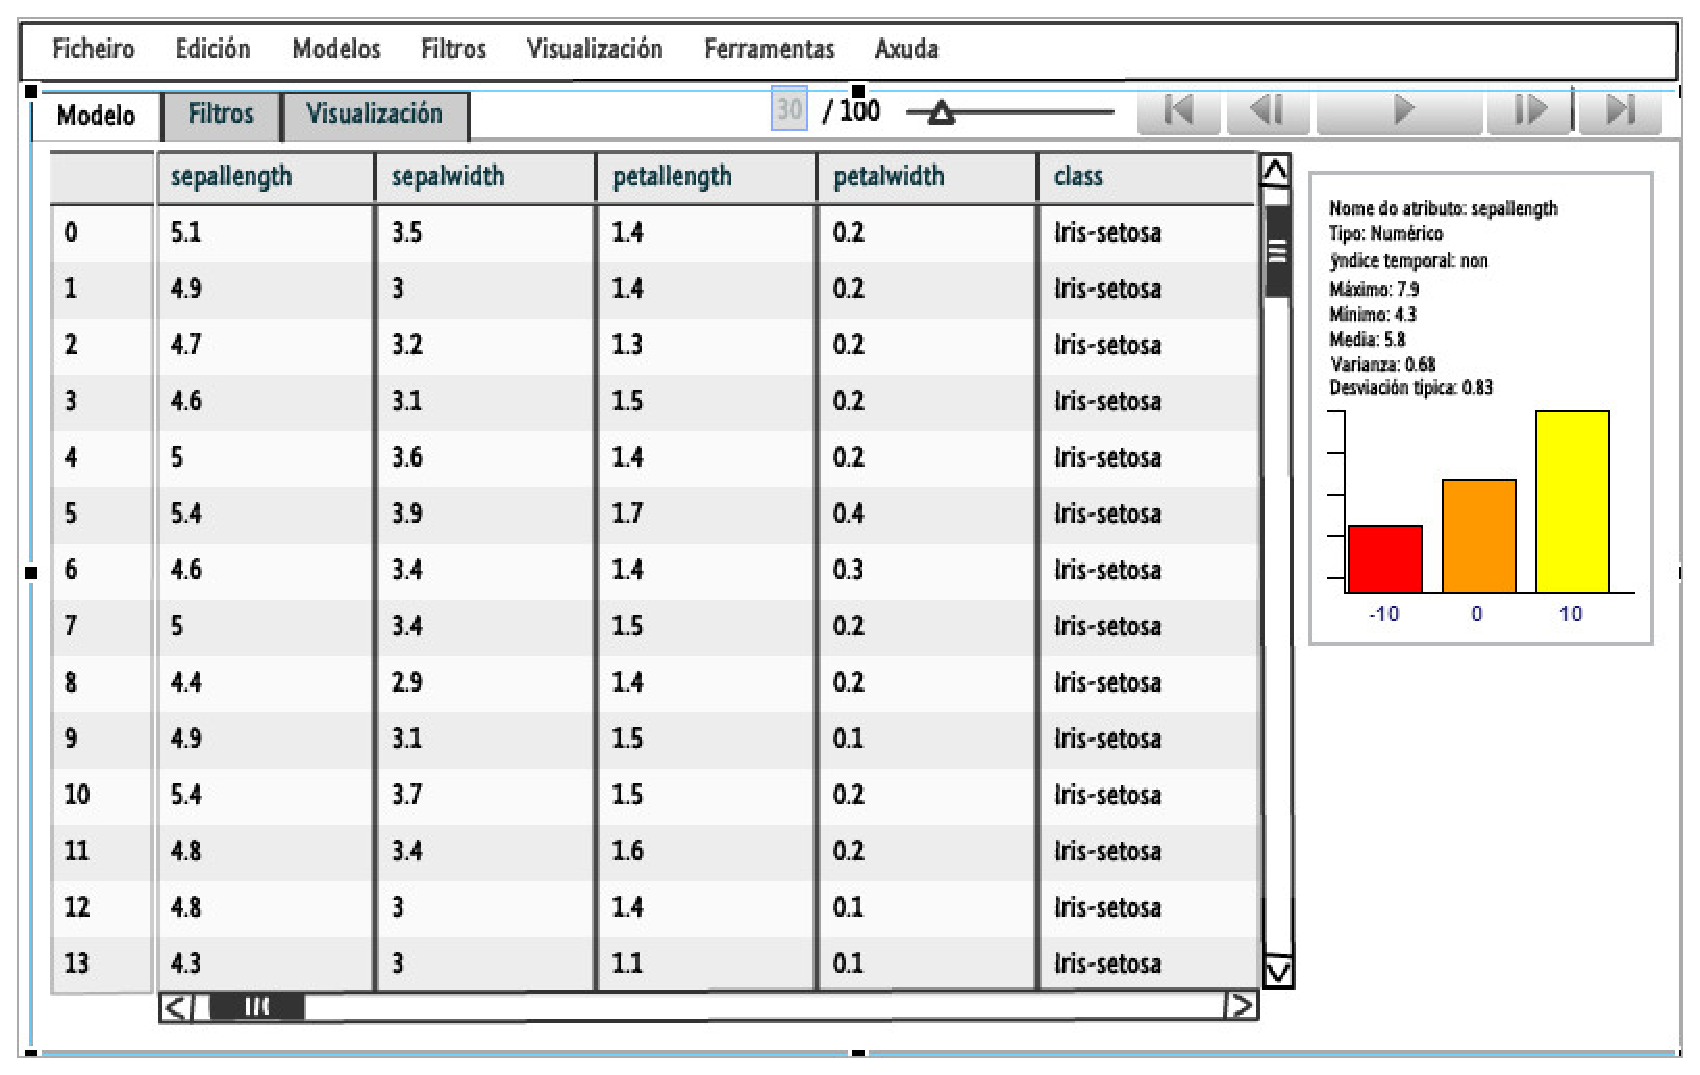
\includegraphics[width=\textwidth,height=\textheight,keepaspectratio]{figuras/Modelo}
\caption{Mockup da sección Modelo}
\label{Modelo}
\end{figure}
\item[Filtros:] \hfill
conterá unha lista de filtros dispoñibles pegada á borde esquerda, e un botón baixo ela que se active cando haxa un filtro desta lista seleccionado, para engadilo. O resto do contedor ocuparao unha secuencia de iconas en fila, facendo referencia aos distintos filtros que se engadiron e aos modelos parciais que temos antes e despois de cada filtro. O mockup desta sección pódese observar na figura \ref{Filtros}.
\begin{figure}
\centering
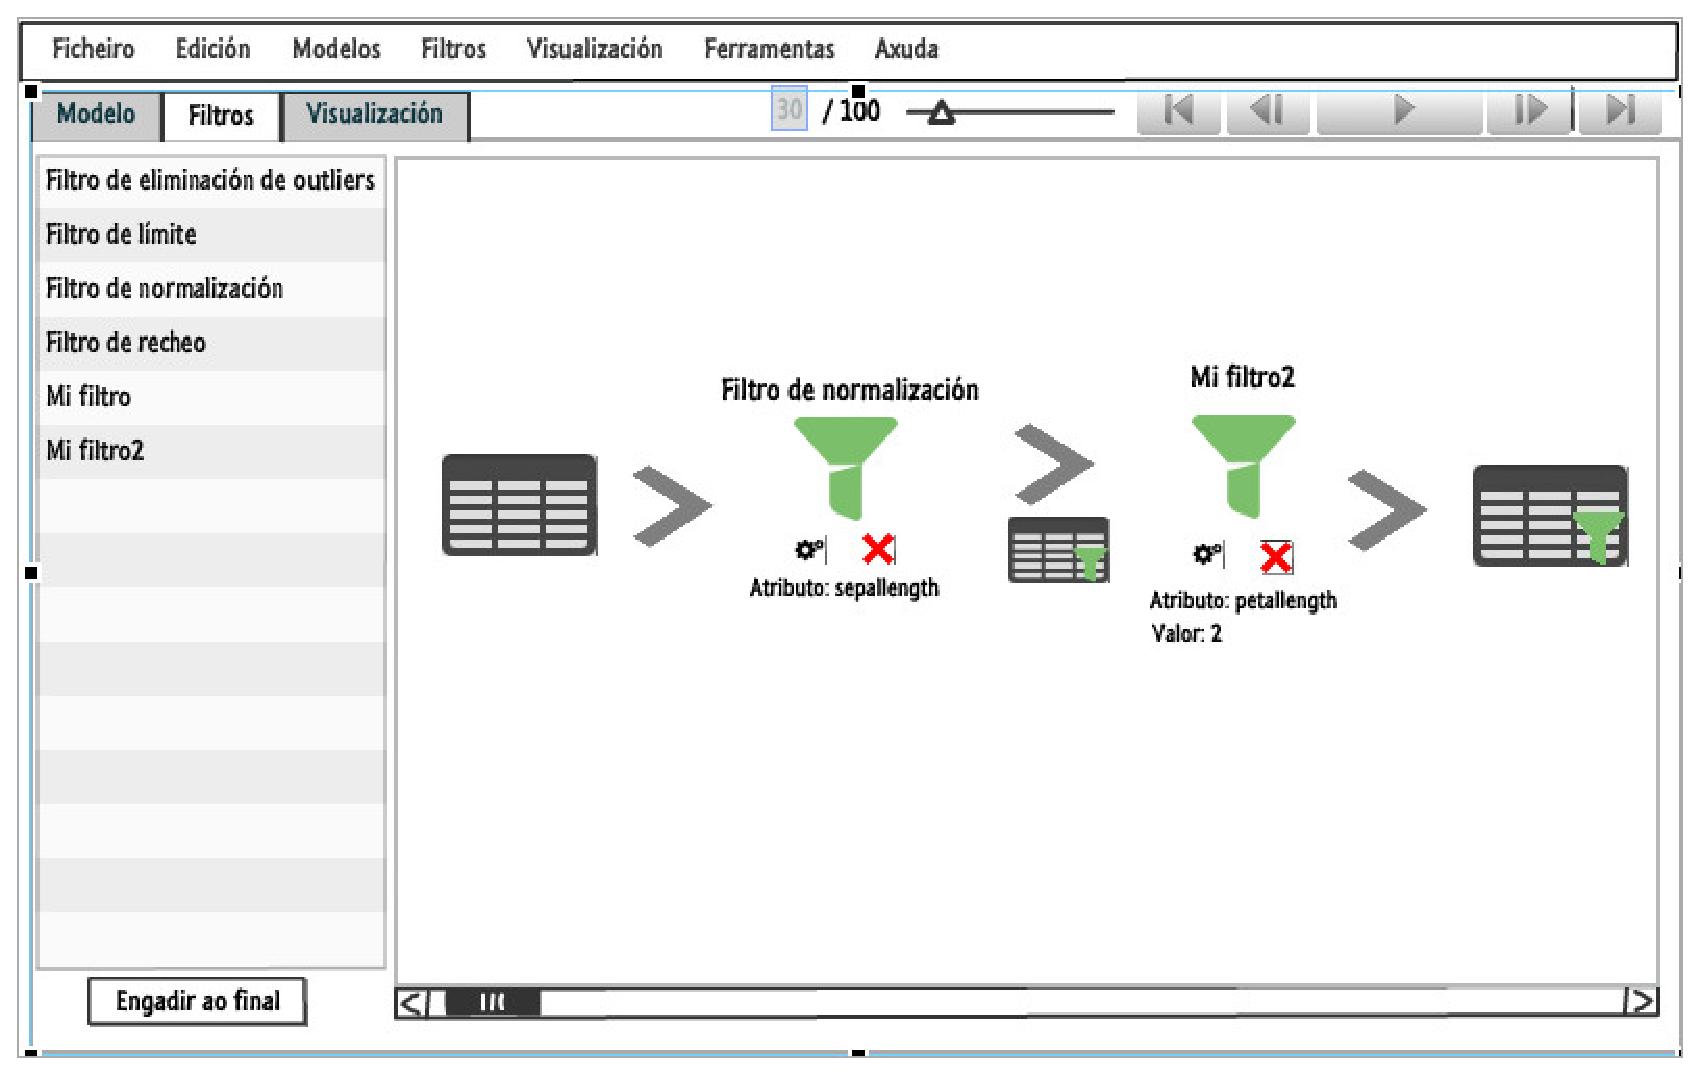
\includegraphics[width=\textwidth,height=\textheight,keepaspectratio]{figuras/Filtros}
\caption{Mockup da sección Filtros}
\label{Filtros}
\end{figure}
\item[Visualización:] \hfill
a totalidade do espacio para esta sección ocuparao un conxunto de diagramas de dispersión organizados baixo unha matriz, de xeito que en cada fila da matriz os diagramas teñan o mesmo atributo para as ordenadas, e en cada columna da matriz os diagramas teñan o mesmo atributo para as abscisas. Cada diagrama disporá dun botón para ser ampliado nunha ventá aparte. Tamén figurarán dentro desta sección aínda que fora do propio contedor (en liña coas lapelas das seccións) 5 botóns asociados a funcións de reprodución (ir a principio, paso atrás, reproducir/pausar, paso adiante e ir ao final), así como un pivote desprazable ao longo dunha barra (moverase conforme se reproduza o experimento) e un indicador do número de elementos xa visualizados e totais. O mockup desta sección pódese observar na figura \ref{Visualizacion}.
\begin{figure}
\centering
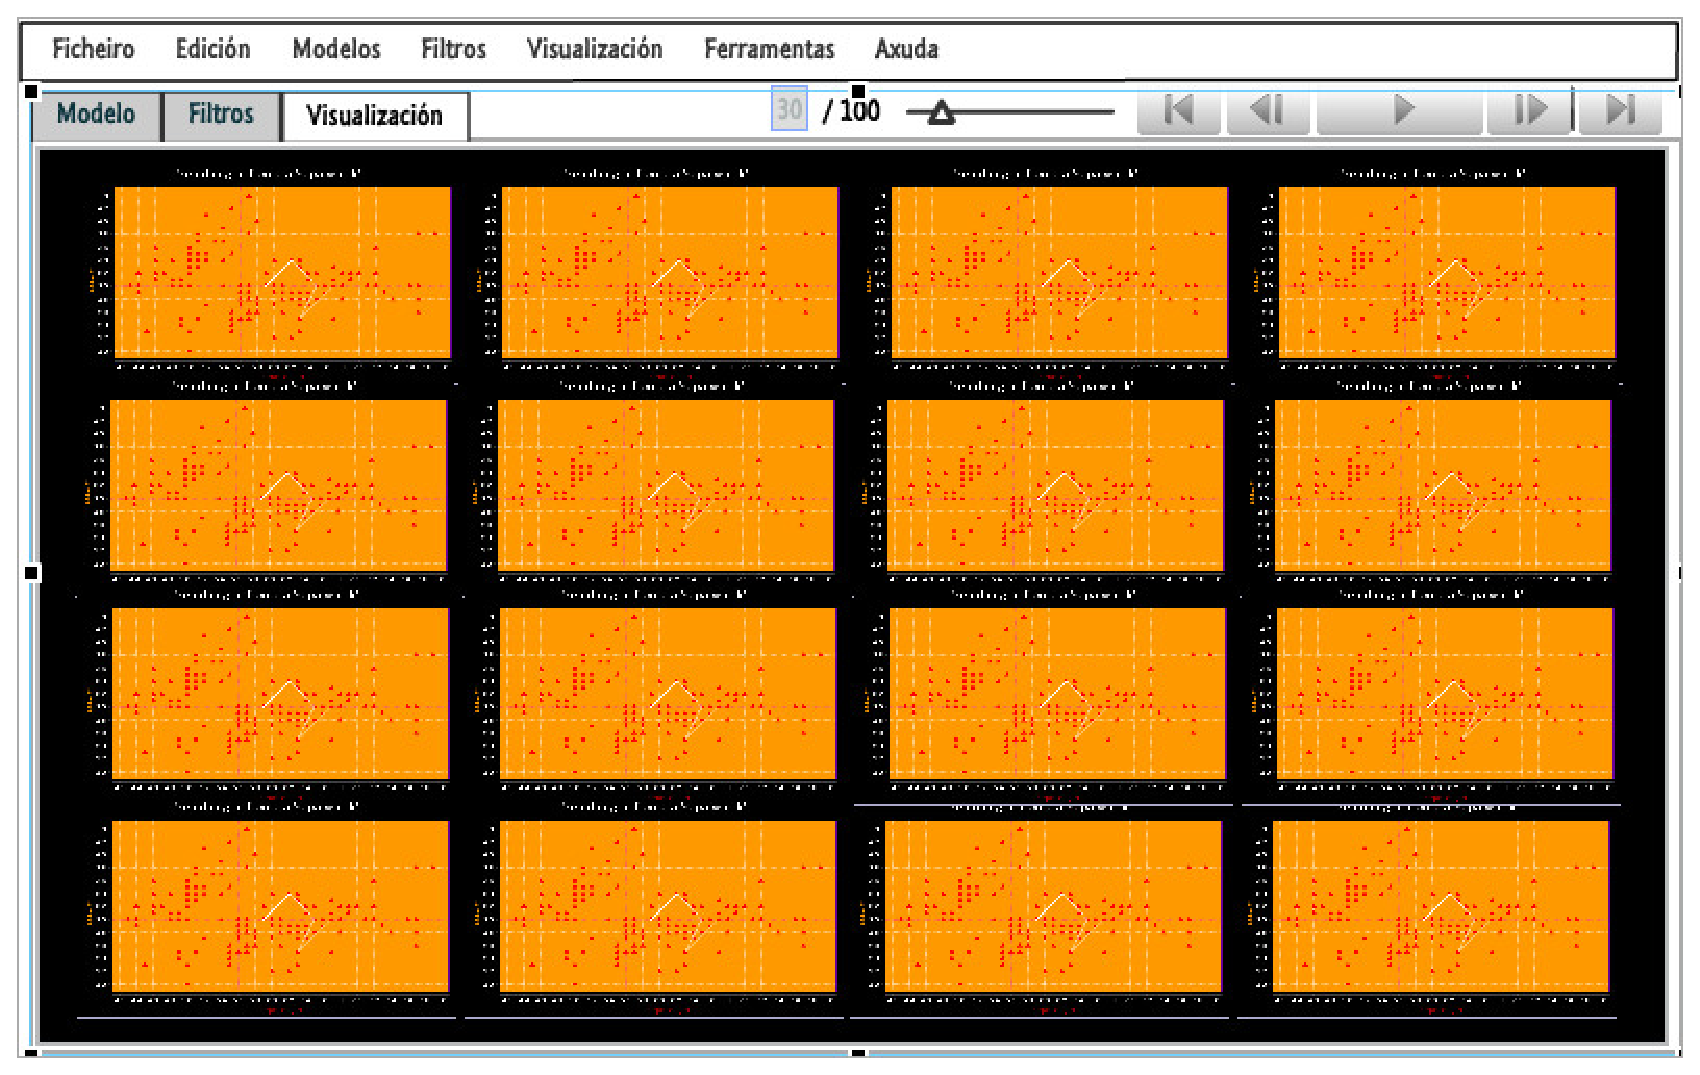
\includegraphics[width=\textwidth,height=\textheight,keepaspectratio]{figuras/Visualizacion}
\caption{Mockup da sección Visualizacion}
\label{Visualizacion}
\end{figure}
\end{description} 

Cada sección foi previamente deseñada a nivel gráfico por medio da ferramenta Lumzy, da cal acabamos de presentar algunhas capturas de pantalla. Para acceder ao mockup e ter unha mínima interacción con el (navegando a través das seccións), podemos utilizar o seguinte enlace (probado a día 10/07/2015):
\\
http://lumzy.com/access/?id=83517845D38CCEEA54A9D6B484A32147

Dada a necesidade do espacio para táboas, listas e sobre todo para a matriz de diagramas de dispersión, adoptouse a medida de desplazar os activadores de case todas as funcionalidades á barra de menús (non operativa no mockup). Prácticamente os únicos botóns que por motivos de usabilidade non podían ser desprazados cara a barra de menús eran os de funcións de reprodución, e de feito tiveron que ir encaixados fóra da propia sección de Visualización sobre a que operan. Entre outros, na barra de menús haberá un título para cada unha das 3 seccións.

Os ítems da barra de menús son os seguintes:

\begin{description}

\item[Ficheiro:] \hfill

\begin{description}

\item[Importar ficheiro:] \hfill
Abre unha ventá cun explorador de ficheiros para seleccionar un arquivo en formato .arff ou .csv. A dirección a ese arquivo mándase ao Controlador como argumento, acompañando a un evento de tipo IMPORTAR\_FICHEIRO.

\item[Exportar ficheiro:] \hfill
Abre unha ventá cun explorador de ficheiros para seleccionar unha ruta e un nome de arquivo en formato .arff ou .csv. A dirección a ese novo arquivo mándase ao Controlador como argumento, acompañando a un evento de tipo EXPORTAR\_FICHEIRO.

\item[Abrir sesión:] \hfill
Abre unha ventá cun explorador de ficheiros para seleccionar un arquivo en formato .jdms. A dirección a ese arquivo mándase ao Controlador como argumento, acompañando a un evento de tipo ABRIR\_SESION.

\item[Gardar sesión:] \hfill
Abre unha ventá cun explorador de ficheiros para seleccionar unha ruta e un nome de arquivo en formato .jdms. A dirección a ese novo arquivo mándase ao Controlador como argumento, acompañando a un evento de tipo GARDAR\_SESION.

\item[Restaurar:] \hfill
Envía ao Controlador un evento de tipo RESTAURAR.

\item[Pechar:] \hfill
Pecha a aplicación JDataMotion.

\end{description}

\item[Edición:] \hfill

\begin{description}

\item[Desfacer:] \hfill
Envía ao Controlador un evento de tipo DESFACER.

\item[Rafacer:] \hfill
Envía ao Controlador un evento de tipo REFACER.

\end{description}

\item[Modelo:] \hfill

\begin{description}

\item[Engadir instancia:] \hfill
Envía ao Controlador un evento de tipo ENGADIR\_DATOS.

\item[Eliminar instancias seleccionadas:] \hfill
Envía ao Controlador un evento de tipo ELIMINAR\_DATOS, acompañado dun array de enteiros que contén os índices das filas do Modelo que están seleccionadas.

\item[Engadir atributo:] \hfill
Envía ao Controlador un evento de tipo ENGADIR\_ATRIBUTO.

\item[Eliminar atributo:] Envía ao Controlador un evento de tipo ELIMINAR\_ATRIBUTO, acompañado do índice do atributo sobre o que se pulsou.

\item[Renomear atributo:] \hfill
Abre un diálogo para introducir o novo nome do atributo pulsado. Envía ao Controlador un evento de tipo RENOMEAR\_ATRIBUTO, acompañado dun array de obxetos co índice do atributo sobre o que se pulsou e o novo nome do atributo.

\item[Mudar nome da relación:] \hfill
Abre un diálogo para introducir o novo nome para a relación. Envía ao Controlador un evento de tipo MUDAR\_NOME\_RELACION, acompañado do novo nome.

\item[Amosar todas as columnas:] \hfill
Volve a amosar todas as columnas que se ocultaron.

\end{description}

\item[Filtros:] \hfill

\begin{description}

\item[Importar filtros:] \hfill
Abre unha ventá cun explorador de ficheiros para seleccionar un arquivo en formato .jdmf. A dirección a ese arquivo mándase ao Controlador como argumento, acompañando a un evento de tipo IMPORTAR\_FILTROS.

\item[Exportar filtros seleccionados:] \hfill
Abre unha ventá cun explorador de ficheiros para seleccionar unha ruta e un nome de arquivo en formato .jdmf. Envía ao Controlador un evento de tipo EXPORTAR\_FILTROS, acompañado dun array de obxetos coa dirección do arquivo e un array de enteiros cos índices dos filtros seleccionados.

\item[Importar filtro dende JAR:] \hfill
Abre unha ventá cun explorador de ficheiros para seleccionar un arquivo en formato .jar. A dirección a ese arquivo mándase ao Controlador como argumento, acompañando a un evento de tipo IMPORTAR\_FILTRO\_DENDE\_JAR.

\end{description}

\item[Visualización:] \hfill

\begin{description}

\item[Engadir ou eliminar scatterplots:] \hfill
Abre unha ventá cunha matriz que enfronta a todos os atributos entre si. Os diagramas de dispersión asociados que se seleccionen ou deseleccionen aparecerán ou desaparecerán da lapela de Visualización.

\item[Establecer atributo nominal representado:] \hfill
Abre un diálogo para seleccionar dunha lista despregable de atributos nominais cal se desexa utilizar para diferenciar os puntos nos diagramas de dispersión.

\item[Configurar reprodutor:] \hfill
Abre un diálogo que permite modificar a orde da reprodución, o paso e a cor e a lonxitude da estela.

\item[Calcular distancia:] \hfill
Abre un diálogo que permite seleccionar dous puntos da lapela de Visualización para calcular a distancia entre eles, segundo unha fórmula editable incluída no diálogo.

\end{description}

\item[Ferramentas:] \hfill

\begin{description}

\item[Idioma:] \hfill

\begin{description}

\item[Galego:] \hfill
Cambia o idioma da aplicación a galego (require reiniciar).

\end{description}

\begin{description}

\item[Español:] \hfill
Cambia o idioma da aplicación a español (require reiniciar).

\end{description}

\begin{description}

\item[Inglés:] \hfill
Cambia o idioma da aplicación a inglés (require reiniciar).

\end{description}

\end{description}

\item[Axuda:] \hfill

\begin{description}

\item[Acerca de:] \hfill
Abre un diálogo con información acerca da aplicación e o seu desenvolvemento.

\end{description}

\end{description}

E a continuación comentaremos as funcionalidades que sí se incorporaron na lapela correspondente ao seu ámbito de actuación:

\begin{description}

\item[Modelo:] \hfill

\begin{description}

\item[Botón secundario nun atributo $\rightarrow$ Tipo:] \hfill

\begin{description}

\item[Numérico:] \hfill
Envía ao Controlador un evento de tipo MUDAR\_TIPO, acompañado dun array de obxectos co índice do atributo sobre o que se pulsou e a constante Attribute.NUMERIC.

\item[Nominal:] \hfill
Envía ao Controlador un evento de tipo MUDAR\_TIPO, acompañado dun array de obxectos co índice do atributo sobre o que se pulsou e a constante Attribute.NOMINAL.

\item[String:] \hfill
Envía ao Controlador un evento de tipo MUDAR\_TIPO, acompañado dun array de obxectos co índice do atributo sobre o que se pulsou e a constante Attribute.STRING.

\item[Data:] \hfill
Envía ao Controlador un evento de tipo MUDAR\_TIPO, acompañado dun array de obxectos co índice do atributo sobre o que se pulsou e a constante Attribute.DATA.

\end{description}

\item[Botón secundario nun atributo $\rightarrow$ Índice temporal:] \hfill
Envía ao Controlador un evento de tipo MUDAR\_INDICE\_TEMPORAL, acompañado do índice do atributo sobre o que se pulsou.

\item[Botón secundario nun atributo $\rightarrow$ Agochar columna:] \hfill
Agocha a columna da táboa correspondente ao atributo no que se pulsou.

\item[Botón secundario nun histograma:] \hfill
Abre un menú contextual no que se pode almacenar o histograma como unha imaxe, copialo, imprimilo ou cambiarlle o zoom ou a escala.

\item[Selección por arrastre dunha área dentro do diagrama de dispersión:] \hfill
Reposiciona e escala o histograma para visualizar a área marcada.

\item[Tecla control + arrastre do diagrama de dispersión:] \hfill
Reposiciona o histograma movendo o lenzo na dirección do cursor.

\item[Roda do rato:] \hfill
Acerca ou afasta o zoom do histograma.

\end{description}

\item[Filtros:] \hfill

\begin{description}

\item[Botón ``Engadir ao final'':] \hfill
Envía ao Controlador un evento de tipo ENGADIR\_FILTRO, acompañado dun array de obxectos co índice que representa a última posición e o filtro que se seleccionou da lista.

\item[Botóns de instancias parciais/finais:] \hfill
Abre unha nova ventá co modelo do experimento ao aplicar os filtros ata ese punto da secuencia.

\item[Botón mover filtro á dereita:] \hfill
Envía ao Controlador un evento de tipo INTERCAMBIAR\_FILTROS, acompañado dun array de obxectos co índice do filtro sobre o que se pulsou este botón e o índice seguinte.

\item[Botón mover filtro á esquerda:] \hfill
Envía ao Controlador un evento de tipo INTERCAMBIAR\_FILTROS, acompañado dun array de obxectos co índice do filtro sobre o que se pulsou este botón e o índice anterior.

\item[Botón configurar filtro:] \hfill
Abre un diálogo con campos para cubrir os valores dos parámetros do filtro (o atributo sobre o que se aplica vai incluído). Envía ao Controlador un evento de tipo CONFIGURAR\_FILTRO, acompañado dun array de obxectos co índice do filtro e o array con estes novos valores.

\item[Botón eliminar filtro:] \hfill
Envía ao Controlador un evento de tipo ELIMINAR\_FILTRO, acompañado do índice do filtro sobre o que se pulsou este botón.

\end{description}

\item[Visualización:] \hfill

\begin{description}

\item[Botón ``Comezar visualización'':] \hfill
Mesmo efecto ca Visualización $\rightarrow$ Engadir ou eliminar scatterplots

\item[Desprazador:] \hfill
Permite moverse a distintos puntos da reprodución, chamando ao método goTo() do ManexadorScatterplots e pasándolle a fracción de tempo na que se situou o pivote do desprazador.

\item[Botón ``Ir ao comezo'':] \hfill
Leva á reprodución ao instante inicial, chamando ao método goTo() do ManexadorScatterplots e pasándolle o valor 0.0.

\item[Botón ``Paso atrás'':] \hfill
Retrocede un paso no reprodución, chamando ao método goToPrevious() do ManexadorScatterplots.

\item[Botón ``Reproducir/Pausar'':] \hfill
Continúa a reprodución no último punto si esta se atopa parada ou pausada, chamando ao método play() do ManexadorScatterplots. Pausa a reprodución si esta está sucedendo, chamando ao método pause() do ManexadorScatterplots.

\item[Botón ``Paso adiante'':] \hfill
Retrocede un paso no reprodución, chamando ao método gotoNext() do ManexadorScatterplots.

\item[Botón ``Ir ao final'':] \hfill
Leva á reprodución ao instante inicial, chamando ao método goTo() do ManexadorScatterplots e pasándolle o valor 1.0.

\item[Botón secundario nun diagrama de dispersión:] \hfill
Abre un menú contextual no que se pode almacenar a imaxe, copiala, imprimila, cambiarlle o zoom ou automatizar a escala durante a reprodución.

\item[Botón secundario nun diagrama de dispersión $\rightarrow$ Propiedades:] \hfill
Este ítem do menú contextual abre unha ventá con opcións de configuración gráfica (colores, fontes, formas, etc.) para aplicar aos diagramas de dispersión desta sección de xeito global. As preferencias establecidas neste menú gardaranse como configuración de usuario.

\item[Selección por arrastre dunha área dentro do diagrama de dispersión:] \hfill
Reposiciona e escala o diagrama para visualizar a área marcada.

\item[Tecla control + arrastre do diagrama de dispersión:] \hfill
Reposiciona o diagrama movendo o lenzo na dirección do cursor.

\item[Roda do rato:] \hfill
Acerca ou afasta o zoom o diagrama de dispersión sobre o que repousa o cursor.

\end{description}

\end{description}

\subsection{Clase JDataMotion}

É a clase que contén o método estático main() da aplicación JDataMotion. Este método é o que se procesa en canto executamos o programa. O seu contido basease unicamente na instanciación dun Modelo, seguido da instanciación dunha Vista. Por último, invoca ao método inicializar(Modelo modelo, boolean visualizar) da instancia de Vista que se creou, pasándolle o modelo como primeiro parámetro e un valor true como segundo.

A responsabilidade do main() remata cando xunta unha vista cun modelo por medio do procedemento inicializar(Modelo modelo, boolean visualizar). Este proceso encárgase de que a vista rexistre a instancia de Modelo que acaba de recibir, e invoca no modelo ao método público addObserver(Observer o), pasándose a vista a sí mesma como parámetro. Como vimos anteriormente, o Modelo estende a clase Observable e por tanto herda os seus métodos. Un destes métodos, o addObserver, permite que as instancias de calquera clase que implemente a interface Observer poidan engadirse como observadoras.

O método inicializar da vista tamén ten a responsabilidade de instanciar un controlador para interactuar co Modelo e que interceda polos dous en transaccións como a xestión e notificación de comandos. Do mesmo xeito, a vista invocará ao método inicializar(Modelo modelo, Vista vista) do controlador, pasando o modelo que recibiu e rexistrou de primeiro argumento, e a si mesma como segundo argumento. O método inicializar que ten o controlador unicamente rexistra as dúas instancias que recibiu, e polas que terá que interceder en varios procesos. Ao rematar, segue a execución do método inicializar da vista, ao cal só lle queda arrancar a interface gráfica se o parámetro visualizar é igual a true. Isto pode non ser de interese no caso da execución de tests de proba, nos que non se desexa interactuar coa nova ventá, se non executar unicamente métodos e comprobar o seu resultado.

Podemos observar mellor o proceso de arranque da aplicación a través da figura \ref{DSarranque}, que contén un diagrama de secuencia con todas as instanciacións e invocacións.

\begin{figure}
\centering
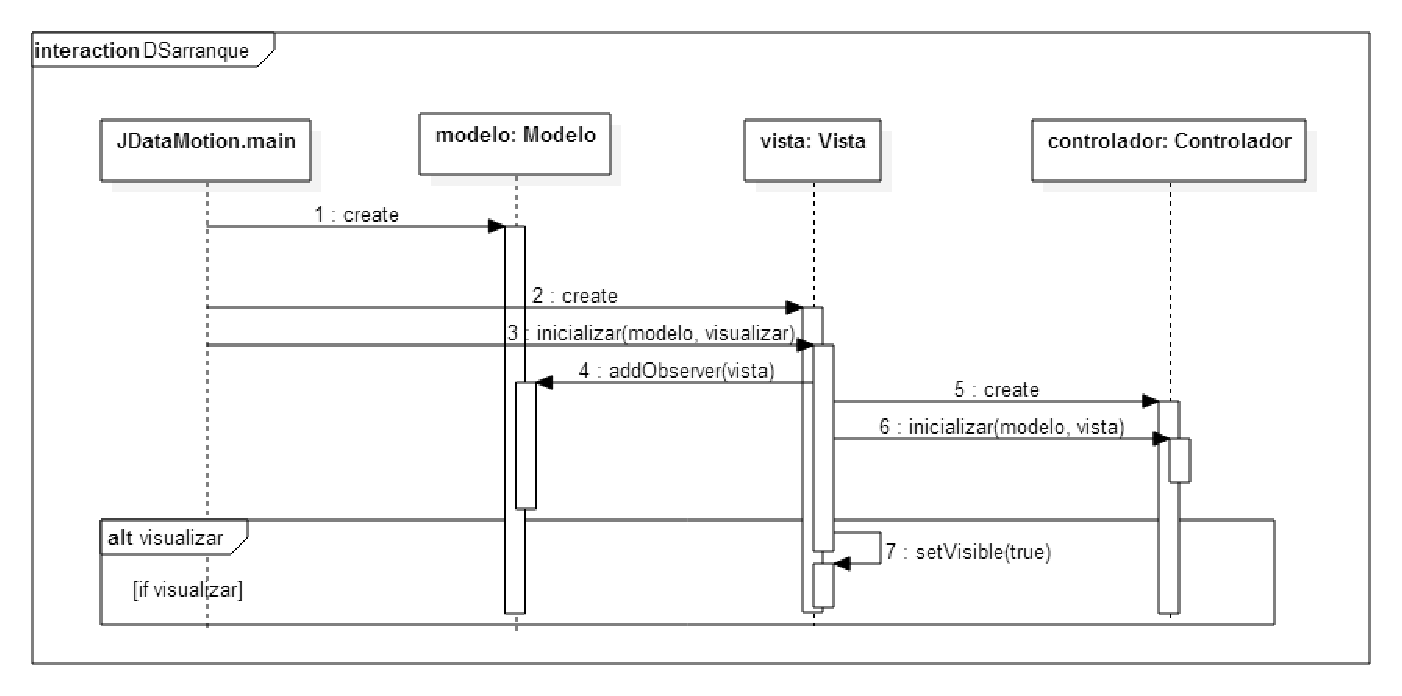
\includegraphics[width=\textwidth,height=\textheight,keepaspectratio]{figuras/DSarranque}
\caption{Diagrama de secuencia do arranque}
\label{DSarranque}
\end{figure}

\subsection{Outros recursos}

As clases das seccións anteriores pertencen ao paquete principal do proxecto JDataMotion. Nel atópanse outros subpaquetes con recursos (clases, ficheiros, imaxes, etc.) que colaboran coas clases principais. A continuación comentaremos cales son:

\begin{description}
\item[jdatamotion.charteditors:] \hfill
Contén clases estendidas para todos os editores gráficos de JFreeChart (menús de configuración gráfica dos diagramas de dispersión). Sobrescribimos algúns métodos destas clases para que lean e escriban cara a configuración almacenada en ficheiro, en vez de aplicar os seus cambios sobre o diagrama que os disparou. 
\item[jdatamotion.comandos:]
Contén todos os comandos susceptibles de ser enviados ao XestorComandos, como xa vimos.
\item[jdatamotion.filtros:]
Contén 4 filtros útiles que xa fornece a propia aplicación:
\begin{description}
\item[FiltroRecheo:] \hfill
Utiliza un parámetro DoubleParameter para cubrir con el as instancias baleiras do atributo sobre o que ten que actuar.
\item[FiltroEliminacionOutliers:] \hfill
Utiliza un parámetro DoubleParameter para eliminar todas as instancias que no atributo sobre o que ten que actuar excedan tantas desviacións típicas da media.
\item[FiltroLimite:] \hfill
Utiliza dous StringParameter, un para saber si ten que actuar sobre un valor límite fixo ou sobre un percentil límite, e outro para saber si ten que actuar sobre valores que excedan ou sobre os que non alcancen ese límite. Tamén utiliza un DoubleParameter que almacenará o valor límite ou o percentil límite, segundo o caso. No atributo sobre o que actúa o filtro, as instancias que queden sinaladas pola configuración anterior cambiarán o seu valor para axustalo ao do límite.
\item[FiltroNormalizacion:] \hfill
Non emprega parámetros. Normaliza en todas as instancias o valor do atributo sobre o que actúa, normalizándoo.
\end{description}
Tamén contén o encapsulador (FilterHandler) de filtros que empregará o Modelo.
\item[jdatamotion.idiomas:]
Contén 3 ficheiros que conteñen as mesmas claves, e en cada un esta clave está relacionada cunha cadea de caracteres nun idioma. Cada ficheiro representa un idioma, e dese xeito pódense traducir mensaxes da aplicación accedendo ao ficheiro do idioma seleccionado e buscando nel o valor da clave.
\item[jdatamotion.imaxes:]
Contén todas as figuras, iconas e demais gráficas que emprega a aplicación na súa interface gráfica.
\item[jdatamotion.sesions:]
Contén a interface Sesionizable da que xa falamos, así como os 3 tipos de sesión nos que o Modelo, a Vista e o Controlador poden almacenar a configuración que desexen salvar dunha sesión a outra.
\end{description}

\section{Deseño de JDataMotion.common}

Este subproxecto contén todo o material que resulta útil tanto para a aplicación JDataMotion coma para outros subproxectos que conteñan filtros válidos para seren importados. O diagrama de clases co seu contido amósase na figura \ref{JDataMotioncommon}.

\begin{figure}
\centering
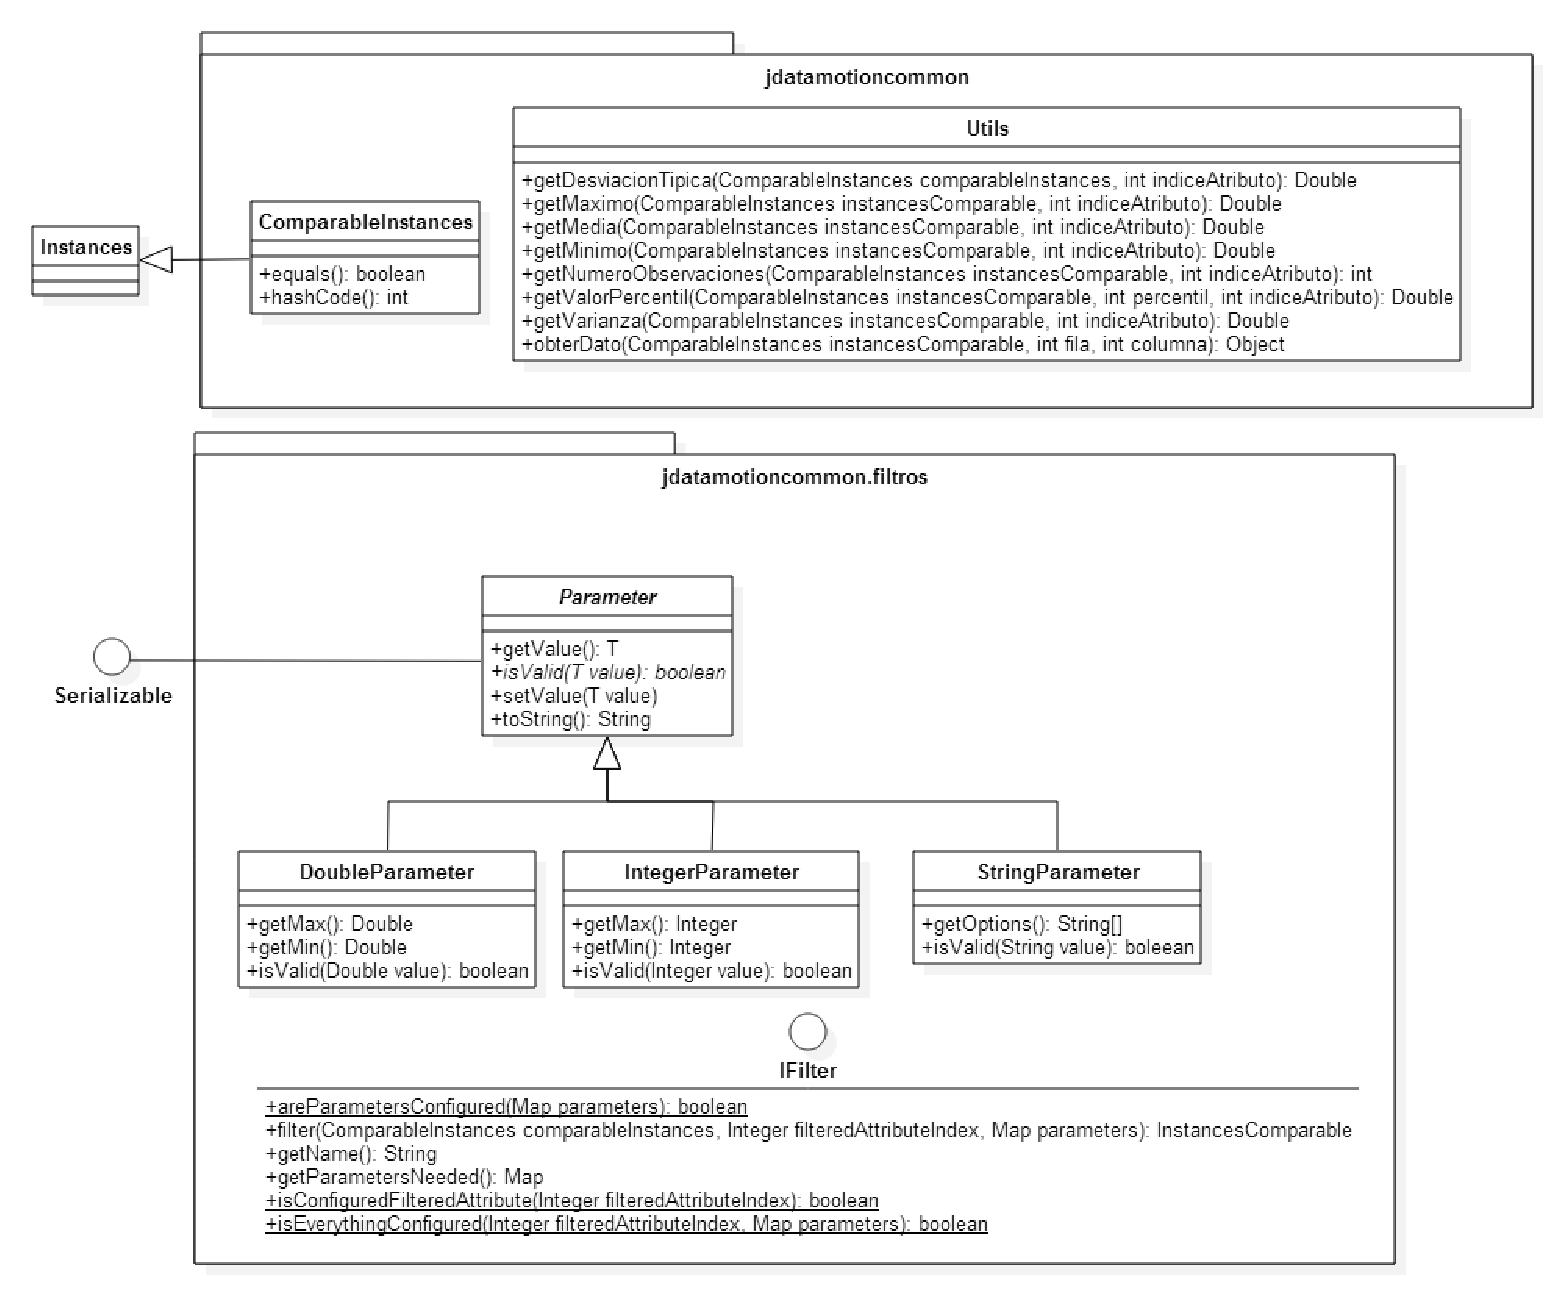
\includegraphics[width=\textwidth,height=\textheight,keepaspectratio]{figuras/JDataMotioncommon}
\caption{Diagrama de clases de JDataMotion.common}
\label{JDataMotioncommon}
\end{figure}

Ademais das clases da figura, o proxecto tamén inclúe as librerías ``weka-dev-3.7.10.jar'', ``weka-dev-3.7.10-javadoc.jar'' e ``weka-dev-3.7.10-sources.jar'', que conteñen respectivamente a interface de programación, a documentación e os códigos fonte do proyecto Weka na súa versión 3.7.10.

O paquete jdatamotioncommon contén a extensión das Instances de Weka que vimos mencionando todo este tempo. Só engaden unha implementación da clase equals(Object o) que nos permite determinar, a partir dos atributos e instancias da clase, que dúas Instances son iguais. Isto axudaranos á hora de realizar os test de proba, comprobando que un obxecto de tipo Instances tras executar un método que o modifica equivale a outro obxecto Instances que nós esperamos.

A clase Utils contén unha batería de métodos estáticos de interese estatístico que resultan moi útiles á hora de programar novos filtros. Case todos reciben como mínimo unha instancia de InstancesComparable e un atributo do que deben extraer un dato (máximo, mínimo, media, varianza, desviación típica, percentil ou o número de observacións).

O paquete jdatamotioncommon.filters contén en primeiro lugar a interface IFilter, que toda clase susceptible de ser importada debe implementar. Os seus métodos descríbense a continuación:

\begin{description}
\item[areParametersConfigured(Map\textless String, Parameter\textgreater{} parameters):] \hfill
Método estático que comproba que os parámetros que necesita o filtro xa teñan un valor asignado.
\item[filter(ComparableInstances comparableInstances, Integer filteredAttributeIndex, Map\textless String, Parameter\textgreater{} parameters):] \hfill
Contén toda a lóxica do filtro. Conta coas comparableInstances que debe filtrar e co índice do atributo sobre o que debe actuar, ademais dos valores dos parámetros que o filtro demandou (o parámetro Map asocia o nome de cada parámetro co parámetro en si). A partir destes inputs, a súa execución devolver unha instancia de InstancesComparable, que consideraremos como filtrada.
\item[getName():] \hfill
Devolve o nome do filtro
\item[getParametersNeeded():] \hfill
Devolve un Map\textless String, Parameter\textgreater{} que conteña os parámetros (baleiros) que o filtro necesita ter cubertos para funcionar, utilizando coma clave para acceder a cada filtro o nome que se lle queira dar. Este nome debe almacenarse no filtro para logo recuperar o parámetro cuberto da estrutura Map.
\item[isConfiguredFilteredAttribute(Integer filteredAttributeIndex):] \hfill
Método estático que comproba que o atributo sobre o que ten que actuar o filtro está definido.
\item[isEverythingConfigured(Integer filteredAttributeIndex, Map\textless String, Parameter\textgreater{} parameters)] \hfill
Comproba que tanto os parámetros teñan un valor asignado como que o índice no que debe actuar o filtro esté definido. Normalmente cando todo isto se cumpra, o filtro poderá ser aplicado.
\end{description}

De todos estes métodos, os únicos que deben ser implementados son filter, getName e getParametersNeeded. O resto son métodos estáticos de utilidade para implementadores e para a propia aplicación.

O paquete jdatamotioncommon.filters tamén contén unha xerarquía de parámetros, que serán os que participen das implementacións de IFilter. A clase Parameter serve para almacenar un valor dun certo tipo T, que é o valor do parámetro. Este valor pode ter unha restrición para ser válido, por iso o método isValid(T value) é abstracto.

As clases que implementarán a Parameter van ser:

\begin{description}
\item[DoubleParameter:] \hfill
É un parámetro que almacena un valor de tipo Double. O seu construtor admite un valor double máximo e outro mínimo para utilizalos na implementación do método isValid(Double value).
\item[IntegerParameter:] \hfill
É un parámetro que almacena un valor de tipo Integer. O seu construtor admite un valor double máximo e outro mínimo para utilizalos na implementación do método isValid(Integer value).
\item[StringParameter:] \hfill
É un parámetro que almacena un valor de tipo String. O seu construtor admite un valor de tipo array de String con opcións válidas para utilizalas na implementación do método isValid(String value).
\end{description}

Estes parámetros son axeitadamente interpretados polo JDataMotion, de forma que á hora de configurar un filtro, para un DoubleParameter ou IntegerParameter apareza unha entrada de formulario que deba ser Double ou Integer e comprendida entre os límites (se os ten). Para os StringParameter, si se especifica un array de String, aparecerá un JComboBox (lista despregable de opcións de Swing).

\section{Deseño de JDataMotion.filters.sample}

Este subproxecto constitúe un exemplo e unha proba da funcionalidade da librería común. O seu deseño, bastante simple, aparece na figura \ref{JDataMotionfilterssample}.

\begin{figure}
\centering
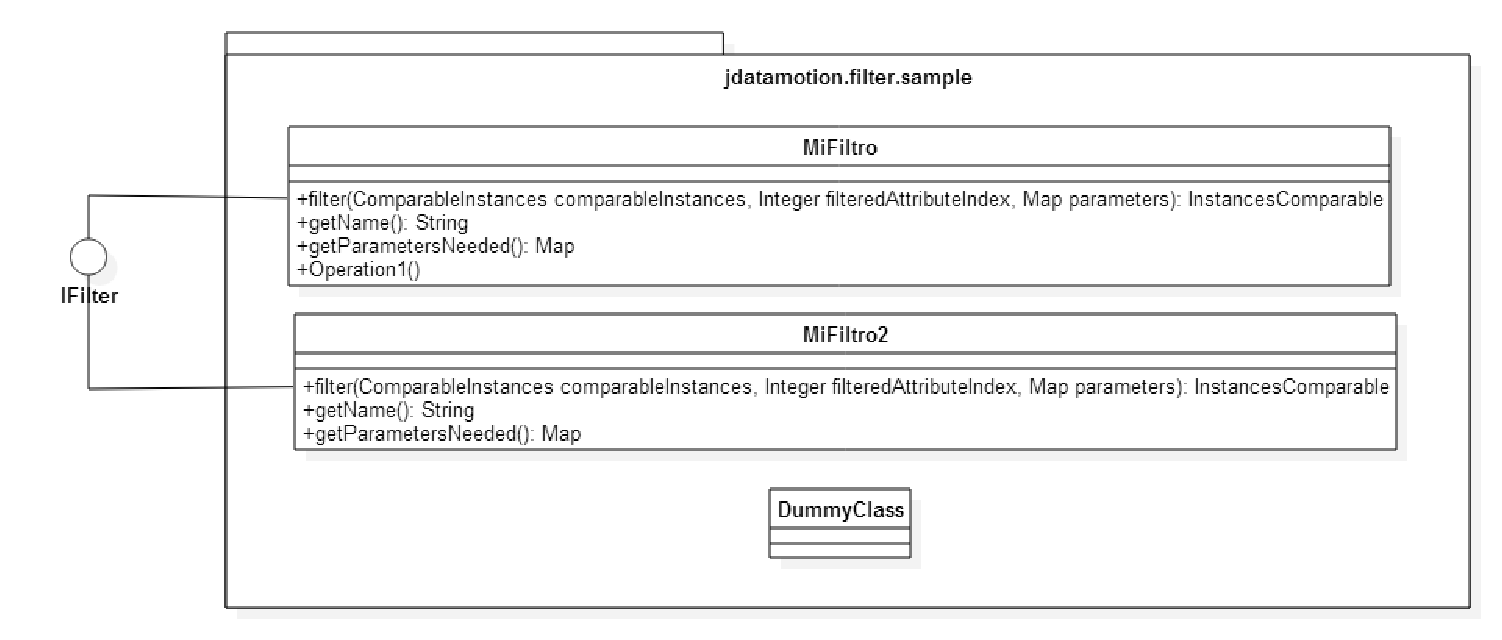
\includegraphics[width=\textwidth,height=\textheight,keepaspectratio]{figuras/JDataMotionfilterssample}
\caption{Diagrama de clases de JDataMotion.filters.sample}
\label{JDataMotionfilterssample}
\end{figure}

É un proxecto constituido por 3 clases:

\begin{description}
\item[MiFiltro:] \hfill
É unha clase que implementa IFilter. Ten un parámetro DoubleParameter de nome ``VALOR'', chámase ``Mi filtro'' e ao filtrar, se todo está correctamente configurado, devolve as instancias do atributo que ten que filtrar multiplicadas por -1 e polo valor do DoubleParameter. Espérase que a importación do .jar admita esta clase.
\item[MiFiltro2:] \hfill
É unha clase que implementa IFilter. Ten un parámetro DoubleParameter de nome ``VALOR'', chámase ``Mi filtro'' e ao filtrar, se todo está correctamente configurado, devolve as instancias do atributo que ten que filtrar multiplicadas por un número aleatorio maior ca 0.0 e menor ca 1.0. Espérase que a importación do .jar admita esta clase.
\item[DummyClass:] \hfill
É unha clase que non implementa IFilter. Espérase que ao importar o arquivo .jar, esta clase sexa descartada.
\end{description}

Imos a ver e comentar a implementación da clase MiFiltro:

\begin{lstlisting}
import java.util.HashMap; //importamos algunhas das clases que facilita Java
import java.util.Iterator;
import java.util.Map;
import jdatamotioncommon.ComparableInstances; // importamos a clase ComparableInstances do paquete jdatamotioncommon
import jdatamotioncommon.filtros.DoubleParameter; // importamos a clase DoubleParameter do paquete jdatamotioncommon.filtros
import jdatamotioncommon.filtros.IFilter; // importamos a interface IFilter do paquete jdatamotioncommon.filtros
import jdatamotioncommon.filtros.Parameter; // importamos a clase ComparableInstances do paquete jdatamotioncommon.filtros
import weka.core.Instance; // importamos a clase Instance de weka.core

/**
 *
 * @author usuario
 */
public class MiFiltro implements IFilter { // MiFiltro implementa a interface IFilter

    private static final String VALOR = "valor"; // nome do parametro que imos utilizar, debemos gardalo e mantelo (modificador final)

		// sobrescribimos o metodo filter
    @Override
    public ComparableInstances filter(ComparableInstances comparableInstances, Integer filteredAttributeIndex, Map<String, Parameter> parameters) {
				// se falta algun parametro por cubrir ou non se defineu o atributo sobre o que se vai actuar, devolvemos as instancias recibidas e o filtro non ten aplicacion (recomendado)
        if (!IFilter.isEverythingConfigured(filteredAttributeIndex, parameters) || !comparableInstances.attribute(filteredAttributeIndex).isNumeric()) {
            return comparableInstances;
        }
				// iteramos ao longo das instancias que recibimos
        Iterator<Instance> it = comparableInstances.iterator();
        while (it.hasNext()) {
            Instance instance = it.next();
						// se a instancia non ten un valor definido no atributo que temos que filtrar, v = null, en caso contrario v toma ese valor
            Double v = instance.isMissing(filteredAttributeIndex) ? null : instance.value(filteredAttributeIndex);
						// establecemos para ese atributo da instancia un valor igual ao que obtivemos (v) multiplicado por -1 e polo valor que se aplicou no parametro
            instance.setValue(filteredAttributeIndex, -(double) parameters.get(VALOR).getValue() * v);
        }
				// devolvemos as instancias filtradas
        return comparableInstances;
    }

		// sobrescribimos o metodo getParametersNeeded
    @Override
    public Map<String, Parameter> getParametersNeeded() {
				// creamos un mapa que relacione String con Parameter
        Map<String, Parameter> p = new HashMap<>();
				// colocamos para o nome do parametro que necesitamos unha instancia sen parametros de DoubleParameter (queremos un parametro de tipo double, sen maximo nin minimo)
        p.put(VALOR, new DoubleParameter());
				// devolvemos o mapa
        return p;
    }

		// sobrescribimos o metodo getName para darlle nome ao filtro
    @Override
    public String getName() {
        return "Mi filtro";
    }

}

\end{lstlisting}